\documentclass[12pt,a4paper,oneside]{report}

% =========================================================
%                 PREAMBLE (ALL FORMATTING HERE)
% =========================================================
\usepackage{booktabs}

% Encoding & language
\usepackage[utf8]{inputenc}
\usepackage[T1]{fontenc}
\usepackage[norsk,english]{babel}
\usepackage{ifxetex}

% Marger
\usepackage[a4paper,
    left=3cm,
    right=2.5cm,
    top=2.8cm,
    bottom=2.8cm]{geometry}


% Bibliography
\usepackage[round]{natbib}

% Math
\usepackage{amsmath, amsfonts, amssymb}

% Typography
\usepackage{microtype}

% Typography
\usepackage{microtype}

% Widow/orphan control
\widowpenalty=10000
\clubpenalty=10000
\raggedbottom


% Graphics & figures
\usepackage{graphicx}
\usepackage{subcaption}
\usepackage[labelfont=bf,labelsep=colon]{caption}
\renewcommand{\figurename}{Fig.}
\usepackage{tikz}
\usetikzlibrary{calc}
\usepackage{float}
\usepackage{placeins}
\usepackage{booktabs}
\usepackage{siunitx}
\usepackage{makecell}

% Layout & spacing
\usepackage{setspace}
\setlength{\parindent}{0pt}
\setlength{\parskip}{1em}
\setlength{\abovecaptionskip}{6pt}
\setlength{\belowcaptionskip}{10pt}

% Section titles
\usepackage{titlesec}
\usepackage{fancyhdr}

% Sidetall-kontroll (Viktig for "X of Y")
\usepackage[pagecontinue=true]{pageslts}

% 1. Stil for FRONT MATTER (romertall, ingen "of X")
\fancypagestyle{frontmatter}{
    \fancyhf{}
    \fancyfoot[R]{\thepage} 
    \renewcommand{\headrulewidth}{0pt}
}

% 2. Stil for MAIN MATTER (arabiske tall, "X of Y")
\fancypagestyle{mainmatter}{
    \fancyhf{}
    \fancyhead[R]{\nouppercase{\leftmark}}
    \fancyhead[L]{\nouppercase{\rightmark}}
    \fancyfoot[R]{\thepage}
    \renewcommand{\headrulewidth}{0.4pt}}

% 3. Stil for kapittel-forsider (fjerner header, beholder "X of Y")
\fancypagestyle{plain}{
    \fancyhf{}
    \fancyfoot[R]{\thepage} 
    \renewcommand{\headrulewidth}{0pt}
}

% Overstyrer standard kapittel-stil
\assignpagestyle{\chapter}{plain}

\renewcommand{\chaptermark}[1]{\markboth{#1}{}}
\renewcommand{\sectionmark}[1]{\markright{#1}}

\titleformat{\chapter}{\normalfont\huge\bfseries}{\thechapter}{1em}{}
\titlespacing*{\chapter}{0pt}{-30pt}{-5pt}

\titleformat{\section}{\normalfont\Large\bfseries}{\thesection}{1em}{}
\titlespacing*{\section}{0pt}{-10pt}{-5pt}

\titleformat{\subsection}{\normalfont\large\bfseries}{\thesubsection}{1em}{}
\titlespacing*{\subsection}{0pt}{0pt}{-5pt}

\titleformat{\subsubsection}{\normalfont\normalsize\bfseries}{\thesubsubsection}{1em}{}
\titlespacing*{\subsubsection}{0pt}{8pt}{-5pt}


% Hyperlinks
\usepackage{xcolor}
\usepackage{hyperref}
\hypersetup{
    hidelinks,
    pdfauthor={Eirik Årdal Hjelm, Sondre Eliassen Haugen},
    pdftitle={Preliminary Study for the Master's Thesis}
}

\ifxetex
    \usepackage{fontspec}
    \newfontfamily{\arial}{Arial}
\else
    \usepackage{helvet}
    \newcommand*\arial{\sffamily}
\fi

\makeatletter
\newcommand{\thesisyear}[1]{\gdef\@thesisyear{#1}}
\newcommand{\credits}[1]{\gdef\@credits{#1}}
\newcommand{\faculty}[1]{\gdef\@faculty{#1}}
\newcommand{\studyprogramme}[1]{\gdef\@studyprogramme{#1}}
\newcommand{\supervisor}[1]{\gdef\@supervisor{#1}}
\providecommand{\@thesisyear}{}
\providecommand{\@credits}{}
\providecommand{\@faculty}{}
\providecommand{\@studyprogramme}{}
\providecommand{\@supervisor}{}
\newcommand{\setmetadata}{%
\ifxetex
        \special { pdf:docinfo <<
            /Title (\@title)
            /Author (\@author)
            /Producer (\@author, Supervision: \@supervisor)
            /Creator (\@author)
            /Subject (Master's Thesis \@thesisyear (\@credits ECTS))
            /Keywords (Norwegian University of Life Science, \@faculty, \@studyprogramme)
         >> }
\else
\pdfinfo{
    /Title (\@title)
    /Author (\@author)
    /Producer (\@author, Supervision: \@supervisor)
    /Creator (\@author)
    /Subject (Master's Thesis \@thesisyear (\@credits ECTS))
    /Keywords (Norwegian University of Life Science, \@faculty, \@studyprogramme)
    }
\fi
}
\makeatother

\title{Exploring Machine Vision for Vehicle and Object Detection in Road Environments}
\author{Eirik Årdal Hjelm, Sondre Eliassen Haugen}
\thesisyear{2026}
\credits{30}
\faculty{Faculty of Science and Technology (REALTEK)}
\studyprogramme{Industrial Economics (INDØK)}
\supervisor{Øyvind Lervik Nilsen}

\input{project/frontpage_nmbu_defs}

% =========================================================
%                 DOCUMENT START
% =========================================================
\begin{document}
\setmetadata

% =========================
% FRONT MATTER (Roman numerals)
% =========================
\pagenumbering{roman}
%\pagestyle{frontmatter} % Stil uten "of X" for front matter

% Forside
\begin{titlepage}
    \thispagestyle{empty}
    \frontpage
\end{titlepage}
 

% Preface 
\cleardoublepage
\chapter*{Preface}
\thispagestyle{frontmatter}
\addcontentsline{toc}{section}{Preface}

% Lim inn preface-tekst her


% Abstract
\cleardoublepage
\chapter*{Abstract}
\thispagestyle{frontmatter}
\addcontentsline{toc}{section}{Abstract}




% Toclist
\cleardoublepage
\pagestyle{frontmatter}
% ---- TOC / Lists ----
\pagestyle{frontmatter}
\cleardoublepage
{
    \setstretch{1}
    \setlength{\parskip}{0pt}
    \tableofcontents
}
\cleardoublepage
\thispagestyle{frontmatter}

\addcontentsline{toc}{section}{List of Figures}
\listoffigures
\cleardoublepage

\thispagestyle{frontmatter}
\addcontentsline{toc}{section}{List of Tables}
\listoftables
\cleardoublepage

% =========================
% MAIN MATTER (Arabic numerals)
% =========================
\cleardoublepage
\pagenumbering{arabic}   % Switch to Arabic numerals
\setcounter{page}{1}     % Start from page 1
\pagestyle{mainmatter}
\assignpagestyle{\chapter}{plain}

\begin{spacing}{1.5}

\chapter{Introduction}
\label{chap:introduction}

\section{Background for the choice of the topic}
\label{sec:background}

% WHY THIS MATTERS
In 2024, Norway registered 124 fatalities and serious injuries in intersection accidents. This was nearly a 30\% increase compared to the average of the previous four years and the highest level since 2015 \citep{trafikksikkerhetsutviklingen2024}. Intersections are among the most demanding traffic environments, where motor vehicles, cyclists, and pedestrians interact within limited space. This creates numerous potential conflict points. 

In current practice, traffic data at intersections is commonly collected through manual registrations. These are short-term, periodic observations that typically last 1-4 hours and are often limited to peak periods \citep{SVV_V714}. This approach is labor-intensive, and captures only a snapshot of traffic conditions, making it poorly suited for characterizing temporal variation across time of day, weekdays, or seasons.
In current practice, traffic data at intersections is commonly collected through manual registrations. These are short-term, periodic observations that typically last 1–4 hours and are often limited to peak periods \citep{SVV_V714}. This approach is labor-intensive and captures only a snapshot of traffic conditions, making it poorly suited for characterizing temporal variation across time of day, weekdays, or seasons.

Norway has pursued a systematic approach to reduce road traffic fatalities over several decades. Annual deaths have fallen from approximately 500 in the 1970s to 87 in 2024 \citep{trafikksikkerhetsutviklingen2024, regjeringen2024_meldst14}. This progress is closely linked to Vision Zero, anchored in the National Transport Plan (NTP) from 2001. The plan aims to eliminate all road traffic fatalities by 2050, with interim targets for 2030, as shown in \autoref{fig:drept_hardt_skadde} \citep{regjeringen2024_meldst14}. However, recent trends suggest Norway is not on track to meet these targets.

\begin{figure}[H]
    \centering
    
\includegraphics[width=0.9\linewidth]{project/images/fatalitiesandinjured.png}
    \caption[Development in road traffic fatalities and serious injuries in Norway]{Development in road traffic fatalities and serious injuries in Norway, with interim targets for 2030 and 2050 \citep{trafikksikkerhetsutviklingen2024}}.
    \label{fig:drept_hardt_skadde}
\end{figure}

Intersections account for a disproportionate share of road traffic casualties. Despite the overall reduction in fatalities and serious injuries since 2001, their share has not declined correspondingly~\citep{svv_trine}. This indicates a continued need for targeted safety measures at these locations, as illustrated in \autoref{fig:prosentandel_kryss}.

\begin{figure}[H]
    \centering
     
\includegraphics[width=0.8\linewidth]{project/images/prosentandel_kryss.png}
    \caption[Percentage of road traffic fatalities and serious injuries occurring at intersections (2001-2024)]
    {Percentage of road traffic fatalities and serious injuries occurring at intersections (2001-2024). Based on data from TRINE \citep{svv_trine}.}
    \label{fig:prosentandel_kryss}
\end{figure}

Norway's long-term transport policy is outlined in the NTP 2025–2036 \citep{regjeringen2024_meldst14}. It emphasizes that digital solutions, new technology, and artificial intelligence can fundamentally change how people and goods are transported. The plan links these tools to improved efficiency and core policy goals such as Vision Zero and reduced environmental impact. In traffic management specifically, it notes that AI can analyze large traffic data streams. It can predict flow and congestion patterns, enabling real-time adjustments of traffic signals, lane usage, and roadside signage.

A central motivation for this thesis is the NTP's explicit recognition that fiscal constraints are tightening. Rising costs in ongoing projects and tighter public budgets are reducing the financial room for new infrastructure investments \citep{regjeringen2024_meldst14}. The plan responds by shifting emphasis toward maintenance, renewal, and solutions that extract greater value from existing assets. This makes a compelling case for examining whether infrastructure already in place, such as fixed roadside cameras, can serve as reliable data sources for traffic monitoring. If existing video installations can be analyzed with AI-based methods, traffic monitoring and safety assessments can be expanded. This, at substantially lower marginal costs than approaches requiring new sensor deployments or repeated manual registrations. Several local authorities abroad are already applying AI to CCTV and video sensors for automated traffic and pedestrian monitoring \citep{ITSKRSComputerVisionCCTV, VivacityValidation2022}.

%What remains unresolved is whether these methods perform reliably enough under real operating conditions to support traffic management decisions. Factors such as variable lighting, weather, occlusion, and camera placement remain insufficiently tested. Existing validation studies are typically conducted under controlled or near-ideal conditions, leaving a gap between reported accuracy and operational deployability. The following section maps this gap in detail and identifies the specific questions this thesis addresses.

\section{Knowledge Gap}
Computer vision (CV) has become an increasingly important component of intelligent transportation systems (ITS). Comprehensive survey studies show that vision-based methods are applied across a wide range of transportation tasks and play a growing role in improving traffic monitoring, safety, and operational efficiency \citep{CVSurvey}.

Previous studies demonstrate that deep learning–based object detection models, particularly YOLO-based architectures, can achieve high accuracy and near real-time performance for vehicle detection and counting. This has been shown in established benchmark datasets and in constrained traffic environments \citep{Everingham10,HuggingFacePascalVOC, Song2019VisionBasedVehicle, smartcities6050134, YOLO-PEL}.

However, the literature also identifies limitations that motivate the research questions in this thesis. \citet{Maity2022LastDecadeVehicleDetection} highlights that many Automatic Vehicle Detection (AVD) studies rely on a limited set of vehicle classes. This motivates \textbf{Research Question 1} on detailed vehicle classification. The same survey further notes that robustness is often not explicitly evaluated under occlusion and dense traffic. Together with reported challenges in adverse lighting and weather, and in small-object/multi-scale detection \citep{DeepLearningTrafficScene2025,YOLO-PEL}, this motivates \textbf{Research Question 2} on performance under varying operational conditions. Finally, calls for practical validation in real-world deployments \citep{YOLO-PEL} and the need for more robust, end-to-end tracking pipelines for complex scenarios \citep{Hassan2024} motivate \textbf{Research Question 3}. This question concerns sustained autonomous operation and reliability over time.


\section{Problem Statement and Research Questions}
\label{sec:rq}

Building on the knowledge gap identified in the previous section, this thesis evaluates how deep learning-based detection and tracking systems can be configured to extract accurate traffic parameters from intersection video. The focus is on detailed vehicle classification and turning movement counts. Existing systems are typically validated on limited vehicle classes and over short evaluation periods. This leaves open questions about performance under varying conditions and sustained autonomous operation during dynamic lighting transitions. The three research questions address these gaps and maintain a clear thread from the literature review to the problem statement.

  
    \textbf{RQ1: How accurately can deep learning-based detection models extract detailed vehicle classification at an intersection?} 
    
    \textbf{RQ2: How do different model configurations (detector + tracker) perform in extracting turning movement counts under varying lighting conditions?}
    
    \textbf{RQ3: To what extent can a vision-based traffic monitoring system operate autonomously over time without manual intervention?}


%Can an adaptive dual-tracker system that automatically switches between optimized day- and nighttime configurations maintain reliable turning movement extraction across lighting transitions without manual intervention?


\section{Scope and limitations}
% WHAT WE WON´T COVER

\subsection*{Scope}
This study is delimited as follows:
\begin{itemize}
    \item \textbf{Geographic:} Analysis of one T-intersection in Norway.

    \item \textbf{Model scope:} Evaluation of YOLO26, the most recent YOLO release, specialized on traffic object detection.

    \item \textbf{Parameters:} Focus on traffic volumes, vehicle composition, turning movements, and the presence of pedestrians.
    
   \item \textbf{Temporal:} Video data collected during February-April 2026, capturing variations across the time of day and weather conditions.
    
\end{itemize}

\subsection*{Limitations}

The study has the following limitations:

\begin{itemize}

    \item \textbf{Camera and privacy constraints:} The traffic camera was not positioned or configured for optimal object detection. Certain areas of the video are intentionally blurred to comply with the General Data Protection Regulation (GDPR) requirements. This may affect detection performance near privacy-masked regions. 
    
    
    \item \textbf{Environmental conditions:} Detection performance may be affected by weather (rain, snow, fog) and lighting conditions (night, shadows).

    \item \textbf{Intersection type:} The pipeline is limited to a T-intersection. Findings may not generalize, as different geometries or camera configurations are unknown.


    \item \textbf{Vulnerable road users:} Low instance counts of cyclists and pedestrians in the dataset limit the reliability of performance estimates for these classes.
    
    
\end{itemize}


\section{Structure of The Thesis}
% HOW THE THESIS IS ORGANIZED~
The thesis is structured as follows: Chapter~\ref{chap:theory} reviews existing traffic registration methods, object detection theory, and relevant literature on YOLO architectures and multi-object tracking. Chapter~\ref{chap:methods} describes the dataset development and the fine-tuning of YOLO26 models for detailed classification. It also presents the implementation of a dual-configuration tracking pipeline using BoT-SORT and ByteTrack. Chapter~\ref{chap:results} presents detection and tracking performance across varying lighting conditions. Chapter~\ref{chap:discussion} discusses the results and addresses the research questions in relation to prior work. Chapter~\ref{chap:conclusion} summarizes the contributions and directions for future research. Supplementary material, including implementation code and raw results, is provided in the appendices.

\chapter{Theory}
\label{sec:theory}
This chapter presents the theoretical framework for AI-based traffic data extraction from intersection video. Section~\ref{sec:traffic_eng} reviews safety trends, design standards, and multimodal data needs. Section~\ref{sec:computer_vision} covers deep learning detection/tracking with focus on the YOLO model. Finally, Section~\ref{sec:literature_review_research_gap} reviews prior work and knowledge gap within the field of automatic object detection.


\section{Traffic Engineering and Intersection Design}
\label{sec:traffic_eng}
This section establishes the traffic engineering context, reviewing safety trends, intersection characteristics, design standards (N100, V121), current data collection methods (V714), and their limitations for detailed multimodal analysis at intersections.
 
\subsection{Traffic Safety Policy and Accident Burden}
\label{sec:safety_policy}

Norway has pursued a systematic approach to reducing road traffic fatalities over several decades. In the 1970s, approximately 500 persons were killed annually; by 2024, this figure had declined to 87~\citep{trafikksikkerhetsutviklingen2024, regjeringen2024_meldst14}. As shown in \autoref{fig:drept_hardt_skadde}, however, recent developments indicate that Norway is currently not on track to achieve the Vision Zero interim targets for 2030.

\begin{figure}[H]
    \centering
    
\includegraphics[width=0.65\linewidth]{project/images/fatalitiesandinjured.png}
    \caption[Development in road traffic fatalities and serious injuries in Norway, with interim targets for 2030 and 2050]
    {Development in road traffic fatalities and serious injuries in Norway, with interim targets for 2030 and 2050. Reproduced from \citep{trafikksikkerhetsutviklingen2024}}

    \label{fig:drept_hardt_skadde}
\end{figure}

Intersections represent a consistently disproportionate share of road traffic casualties. Despite the overall reduction in total fatalities and serious injuries since 2001, the intersection share has not declined correspondingly \citep{svv_trine}, indicating a continued and specific need for targeted safety measures at these locations, as illustrated in \autoref{fig:prosentandel_kryss}.

\begin{figure}[H]
    \centering
    
\includegraphics[width=0.8\linewidth]{project//images/prosentandel_kryss.png}
    \caption[Percentage of road traffic fatalities and serious injuries occurring at intersections (2001-2024)]
    {Percentage of road traffic fatalities and serious injuries occurring at intersections (2001-2024). Based on data from TRINE \citep{svv_trine}.
}
    \label{fig:prosentandel_kryss}
\end{figure}

The societal costs associated with these accidents are substantial. Applying unit cost rates from the V712 \textit{Consequence Analysis} \citep{svv_v712_2025}, intersection accidents incurred approximately 4.1~billion NOK in societal costs in 2024 alone, with cumulative costs exceeding 128~billion NOK over the period 2001--2024. These figures underscore the economic, in addition to the human, imperative for improved road safety at intersections.

\subsection{Intersection Types and Safety Characteristics}
\label{sec:intersection_types}

Intersections can be classified into several geometric configurations, with T-intersections (three-legged) and X-intersections (four-legged) being the most common forms. Their safety characteristics differ significantly due to variations in the number of conflict points — locations where vehicle trajectories intersect, merge, or diverge. As illustrated in \autoref{fig:konfliktpunkter}, a T-intersection contains 9 conflict points compared to 32 in an X-intersection \citep{svv_V121}, resulting in a substantially lower collision probability and lower average accident costs per incident.

\begin{figure}[H]
    \centering
    
\includegraphics[width=0.8\linewidth]{project/images/Konfliktpunkter.png}
    \caption[Conflict points in T-intersections and X-intersections]{Conflict points in T-intersections (9 points) and X-intersections (32 points). Source: N-V121 \citep{svv_V121}, p. 7}
    \label{fig:konfliktpunkter}
\end{figure}

Between 30 and 40 percent of all police-reported accidents occur at intersections and driveways \citep{svv_V121}, with the most severe incidents involving vehicles on crossing trajectories or conflicts with pedestrians and cyclists. Average societal costs per personal injury accident vary by intersection type: 2.0 million NOK for T-intersections, 1.8 million NOK for X-intersections, and 1.3 million NOK for roundabouts (2009 prices) \citep{svv_V121}.


\subsection{Geometric Design Requirements}
\label{sec:geometric_design}
The Norwegian Public Roads Administration's handbooks \textit{N100: Road and Street Design} \citep{svv_n100} and \textit{N-V121: Geometric Design of Road and Street Intersections} \citep{svv_V121} establish the regulatory framework for road and intersection design in Norway. These standards specify geometric requirements based on key traffic parameters, including traffic volumes, vehicle composition, turning movements, and the presence of pedestrians and cyclists.

A \textit{design vehicle} is the vehicle type used as the basis for determining geometric design parameters such as turning radius, lane width, and corner radii \citep{svv_n100}. According to N100, the selected design vehicle defines both physical dimensions (length, width) and expected driving behaviour, including lane discipline, allowable speeds through intersections, and whether encroachment into adjacent lanes or reversing is permitted. Intersections dimensioned for passenger cars must nevertheless remain accessible to trucks, albeit through less favorable driving maneuvers \citep{svv_n100}. 

\autoref{fig:design_vehicle} illustrates this principle, showing the swept path of heavy vehicles through an urban intersection designed primarily for cars. In accordance with N100 requirement 5.2--2, truck accessibility is ensured, although it requires unconventional driving behaviour.

\begin{figure}[H]
    \centering
    
\includegraphics[width=1\linewidth]{project/images/design_vehicle.png}
    \caption[Swept path comparison between heavy vehicles and passenger cars through an urban intersection]{Swept path comparison between heavy vehicles and passenger cars through an urban intersection. Reproduced from \citep{NACTO_DesignVehicle}.}
    \label{fig:design_vehicle}
\end{figure}

In urban intersections, pedestrian and cyclist safety requires particular attention due to frequent conflicts with motorized traffic \citep{svv_V121}. Compact geometric designs with tight corner radii and constrained lane widths serve dual purposes: forcing drivers to reduce speed while shortening crossing distances for vulnerable road users. The selected design vehicle must therefore reflect dominant traffic composition and intended road function, while accommodating less frequent vehicle types through alternative maneuvers. Geometric design thus requires balancing motorized vehicle requirements against the safety needs of pedestrians and cyclists.

Accurate traffic data capturing vehicle composition, turning movements, and vulnerable road users presence are therefore essential for verifying whether intersection designs function as intended and meet the requirements outlined in N100 and V121.

\subsection{Traffic Data Collection for Intersections}
\label{sec:traffic_data}
Traffic data form the foundation for evidence-based decisions in road infrastructure planning, design, and safety analysis, capturing key metrics such as vehicle volumes, turning movements, speeds, and multimodal interactions (vehicles, cyclists, pedestrians) \citep{SVV_V714}. In Norway, the Norwegian Public Roads Administration's Handbook V714 \textit{Traffic Data Guidelines} regulates collection and management \citep{SVV_V714}. Data are gathered via manual or automated methods, each with strengths suited to specific applications \citep{SVV_V714}.

In Norway, the collection and management of traffic data are regulated by the Norwegian Public Roads Administration through Handbook V714: Traffic Data Guidelines \citep{SVV_V714}. Traffic data can be collected using both manual and automated methods, depending on the purpose, required accuracy, and temporal coverage \citep{SVV_V714}.

\subsubsection{Manual Traffic Counts:}

Manual counts involve personnel recording data on forms or digital devices (e.g., PDAs, laptops). \citep{SVV_V714} They excel at detailed, short-term observations (typically 1--4 hours) during peaks, providing turning movements and multimodal data with high accuracy under controlled conditions. \citep{SVV_V714} However, they cannot capture full temporal variations (daily/weekly/seasonal) without excessive cost and labor. \citep{SVV_V714}

\subsubsection{Automated Traffic Counts:}

\begin{itemize}
    \item \textbf{Inductive loops:} Insulated wire loops installed in saw-cut slots in the pavement so that they form an electrical coil. When a vehicle passes over, the metal mass disturbs the electromagnetic field above the loop, and this change is used to register the vehicle’s presence as a detection event or count \citep{SVV_V714}.

    \item \textbf{Radar sensors:} Employ the Doppler effect to detect vehicle speed and direction by transmitting pulses and analysing the frequency shift in reflected signals from approaching or receding objects. They register traffic volume and speed in both directions \citep{SVV_V714}.

    \item \textbf{Piezoelectric cable:} Pressure sensitive wires that generate measurable voltage proportional to applied force, detecting vehicle axles when two cables are laid transversely across the lane at fixed spacing.  They can be embedded in pavement like inductive loops or glued on surface for short-term use, enabling accurate speed, weight (WIM), axle counts, and spacing measurements \citep{SVV_V714}. 
    
    \item \textbf{Pneumatic hoses:} Rubber hoses that are temporary detectors mounted across the road surface. When a vehicle axle passes over the tube, the generated air pulse is converted into an electrical signal in the recording unit \citep{SVV_V714}

\end{itemize}

Manual and automated methods complement each other in intersection data collection. Manual counts are well suited for short-term, detailed observations during peak periods, while automated methods enable continuous monitoring and capture traffic patterns across different temporal scales \citep{SVV_V714}. In Norway, inductive loops are the most widely used detection method, followed by radar and pneumatic hoses. However, all methods have inherent strengths and limitations related to accuracy, installation, maintenance, and data type.

Manual methods provide detailed snapshots for complex scenarios like intersections, while automated sensors enable continuous monitoring across temporal scales. \citep{SVV_V714} Inductive loops dominate in Norway's system, followed by radar/hoses, but all have context-specific limitations in accuracy, durability, and multimodal coverage \citep{SVV_V714}.

\subsubsection*{LiDAR}
In addition to the standardized methods described in Handbook V714, emerging sensing technologies such as LiDAR (Light Detection and Ranging) have been explored in research and pilot contexts. LiDAR is an active sensing technology capable of detecting surrounding objects with high spatial accuracy over relatively long measurement distances. During operation, the sensor emits laser pulses and records the reflected signals to generate three-dimensional point clouds representing the X, Y, and Z coordinates of objects in the environment. Unlike passive optical systems, LiDAR can operate continuously and is largely independent of ambient lighting conditions \citep{Lv2019_LiDAR}.

While LiDAR is not part of the Norwegian Public Roads Administration’s standard traffic counting infrastructure, it has been tested in pilot projects, including the Borealis ITS test corridor on E8 in Skibotndalen and short-term intersection trials combining mobile cameras and LiDAR for movement analysis in urban environments \citep{SVV_ITS_teststrekninger, SVV_2025_kryss_lidar_test}. Research studies further demonstrate that static roadside LiDAR combined with deep learning models can enable detailed scene understanding and road user classification in intersection settings \citep{LiDAR_IEEE}.

\subsection{Limitations of Current Methods}
\label{sec:limitations_methods}
While Handbook V714 establishes comprehensive standards for traffic data collection in the Norwegian Public Roads Administration (SVV), current methods, both manual and automated, have significant limitations for detailed intersection monitoring \citep{SVV_V714}.

\subsection*{Manual Traffic Counts}
Manual traffic counting can provide high accuracy for specific parameters under controlled conditions, but it faces fundamental limitations that restrict its applicability. Observation periods are typically constrained to 1–4 hours \citep{SVV_V714}, preventing the capture of temporal variations across different times of day, days of the week, or seasonal patterns. Such variations are essential for comprehensive intersection analysis and design. 

In addition, manual counting is labour-intensive and therefore economically demanding. The method is also prone to human error, particularly in complex traffic environments with high volumes or multiple turning movements. As a result, manual counts primarily provide short-term snapshots rather than continuous, behavioural datasets.

\subsection*{Automated Traffic Counts}

\textbf{Inductive loop detectors} generally provide high accuracy for traffic volume measurements under normal operating conditions \citep{SVV_V714}. However, in low-speed situations such as congestion or queuing, vehicles stopping or moving slowly over the loop may lead to underestimation or misclassification. The embedded installation in the pavement makes the system vulnerable to external factors. In Norwegian conditions, winter maintenance operations, including road milling and snow removal, can damage the loops, resulting in costly repairs and temporary data loss. Furthermore, inductive loops primarily measure aggregated vehicle parameters at fixed points and provide limited classification detail.

\textbf{Radar sensors} are used to measure traffic volume and speed in both directions of travel \citep{SVV_V714}. In high density traffic, overlapping targets and signal interference may reduce detection accuracy. Although radar systems can support vehicle classification, performance depends heavily on calibration and environmental conditions, and classification capabilities are therefore limited in practice. Radar sensors must also be carefully positioned to avoid queue areas near intersections, where standing or slow-moving vehicles may affect measurement reliability. While radar technology can technically detect pedestrians and cyclists, such applications are rarely implemented in operational traffic monitoring.

\textbf{Piezoelectric cables} are primarily used for short-term applications, typically lasting only a few days due to their installation method. The cables are exposed to mechanical wear and generally do not function reliably for extended periods. Winter conditions further reduce measurement reliability, and maintenance operations such as snow plowing increase the risk of damage. Installation and removal often require temporary road closure, leading to operational disruptions.

\textbf{Pneumatic road tubes} are relatively simple and cost-effective but have several limitations. When a single tube is installed, the system registers axle counts rather than individual vehicles, which may result in overestimation of traffic volumes for heavy vehicles. With two tubes, additional parameters such as speed and direction can be derived; however, the method remains suitable only for short-term measurements due to rapid wear and vulnerability to winter conditions. As with piezoelectric cables, installation typically requires temporary road closure.

\subsubsection*{Overall Limitations}

Overall, traditional traffic data collection methods are primarily designed to measure aggregated vehicle-based parameters at fixed points. While they provide reliable traffic volumes and speed estimates, they offer limited insight into spatial traffic dynamics, turning trajectories, multimodal interactions, and behavioural patterns at intersections. Detection of pedestrians and cyclists is either limited or not operationally implemented, and interaction-based safety indicators cannot be derived from conventional sensor data. 

As a consequence, important aspects of intersection performance and safety remain largely unobserved in existing traffic datasets. This structural gap motivates the investigation of AI-based computer vision methods, which may enable automated and scalable extraction of detailed traffic metrics from existing camera infrastructure.


\subsection{International Practice}
\label{sec:international_practice}
Internationally, Germany provides a well-documented example of formal approval regimes for automated traffic counting and vehicle classification. Systems such as the TOPO platform are certified by the Federal Highway Research Institute (BASt) and are based on non-intrusive sensor technologies, including radar and LiDAR, rather than video-based deep learning. These systems classify vehicles according to classes defined in German technical specifications and are approved for use in official traffic counting \citep{RTBGmbHCoKG2019}.

In the United States, traffic data collection relies on a mix of technologies with limited use of video-based systems. Historically, traditional video image detection (VID) systems have been capable of collecting and analysing standard traffic data, but with important limitations: their classification ability is largely restricted to daylight operation, and they typically only support three to five length-based vehicle classes, making them unsuitable for axle-based schemes such as required by the FHWA \citep{FHWA2014VID}. Recent guidance from the Washington State Department of Transportation indicates that inductive loops and pneumatic tubes remain the dominant technologies for traffic counting and vehicle classification, with video not established as a standard method \citep{WSDOT2024}. At the same time, some local authorities are beginning to apply artificial intelligence to existing CCTV infrastructure for traffic and pedestrian monitoring, demonstrating a potential pathway for cost-effective use of computer vision without new sensor deployments \citep{ITSKRSComputerVisionCCTV}

In the UK, local authorities have documented the operational use of video-based traffic sensors combined with artificial intelligence. Cambridgeshire County Council reports the deployment of Vivacity sensors to collect classified traffic flow data for transport planning and decision-making, using AI applied to video to count and classify vehicles, pedestrians, and cyclists \citep{VivacityValidation2022}. 

These examples indicate that while video-based and AI-enabled systems are increasingly used for traffic monitoring and data collection, this is typically in combination with other technologies or within pilot and local operational contexts. No evidence has been identified of national road authorities relying solely on video-based data for vehicle classification as a normative basis for traffic data used in design or dimensioning.

\section{Deep Learning and Computer Vision}
\label{sec:computer_vision}

\subsection{Theoretical Foundations of Machine Learning and Computer Vision}
\label{sec:ml_cv}

Machine learning (ML) is a subfield of artificial intelligence in which algorithms infer decision logic directly from data, rather than relying on hand-crafted rules \citep{Goodfellow-et-al-2016}. Within this field, computer vision (CV) concerns the automatic interpretation of visual information from images and video, enabling the extraction of semantic content, including object identity, spatial position, and motion, from raw pixel data \citep{Szeliski2010}.

Recent advances in deep learning have substantially improved the robustness of computer vision systems to real-world variability in illumination, viewpoint, and occlusion, by learning hierarchical feature representations from large-scale image datasets \citep{LeCun2015}. These properties are particularly relevant for traffic monitoring in complex outdoor environments, where conditions change continuously and manual data collection is both costly and inconsistent.

Vision-based analysis tasks are commonly categorised into three progressively more complex problem types, each building on the previous, as illustrated in \autoref{fig:Classification}. \textbf{Image classification} assigns a single semantic label to an entire image but provides no spatial information about object location \citep{Krizhevsky2012}. \textbf{Object detection} extends this by simultaneously identifying object categories and localising each instance through bounding boxes, a capability that is essential for characterising the spatial distribution of vehicles, cyclists, and pedestrians at intersections \citep{Ma2024}. \textbf{Object tracking} further associates detections across consecutive video frames, enabling the reconstruction of object trajectories over time \citep{Bewley2016}. For intersection monitoring, tracking is the critical step that transforms frame-level detections into actionable traffic data, including turning movement counts, vehicle class distributions, and downstream conflict event identification.

\begin{figure}[H]
    \centering
    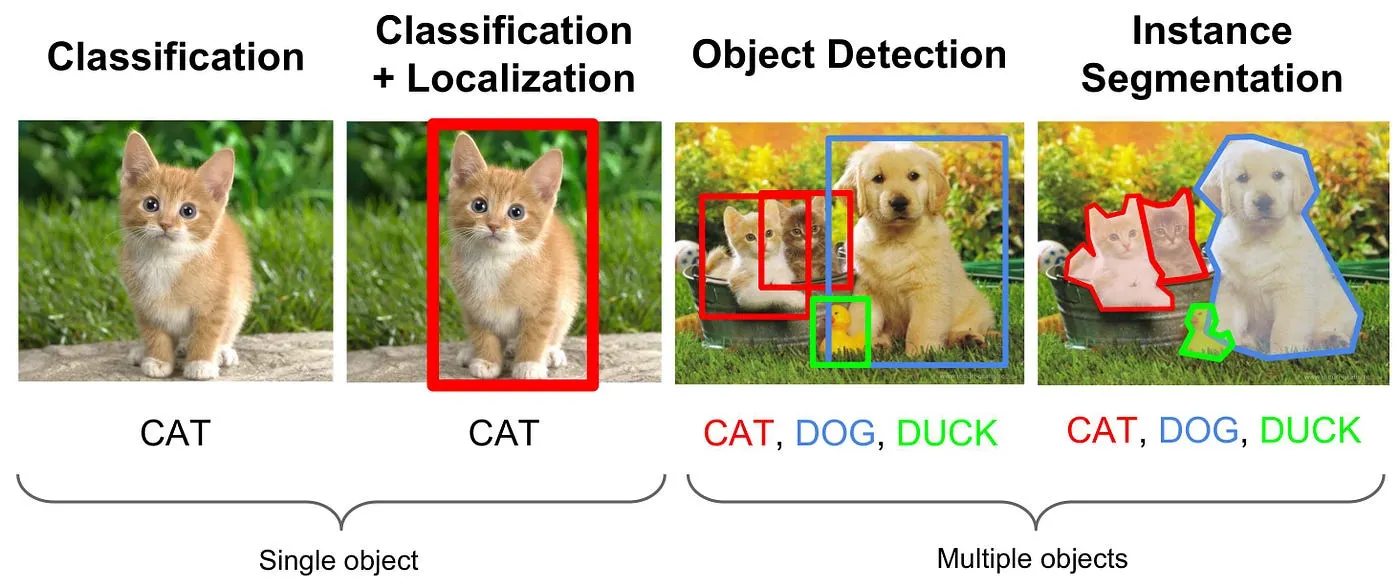
\includegraphics[width=0.7\linewidth]{images/Classification.png}
    \caption{Conceptual illustration of the differences between image classification, object detection, and object tracking in computer vision.}
    \label{fig:Classification}
\end{figure}

\subsection{Deep Learning and Convolutional Neural Networks}
\label{sec:dl_cnn}

Deep learning is a class of machine learning methods based on artificial neural networks with multiple hidden layers, enabling the learning of complex, hierarchical representations from large-scale data \citep{Goodfellow-et-al-2016}. In contrast to shallow models, deep learning architectures are particularly effective for high-dimensional inputs such as images and video, where relevant features must be extracted directly from raw pixel data rather than engineered manually.

Convolutional neural networks (CNNs) represent the foundational deep learning architecture for computer vision. CNNs exploit the spatial structure of image data through convolutional layers, which apply learnable filters across local regions of the input. This mechanism allows CNNs to detect spatially local patterns, including edges, textures, and shapes, at any position in the image, a property known as translational equivariance \citep{LeCun2015}. A typical CNN architecture combines convolutional layers for feature extraction, nonlinear activation functions such as the Rectified Linear Unit (ReLU) to enable the modelling of complex decision boundaries \citep{Nair2010}, and pooling layers that reduce spatial resolution to increase robustness to minor positional variations and reduce computational cost.

\begin{figure}[H]
    \centering
    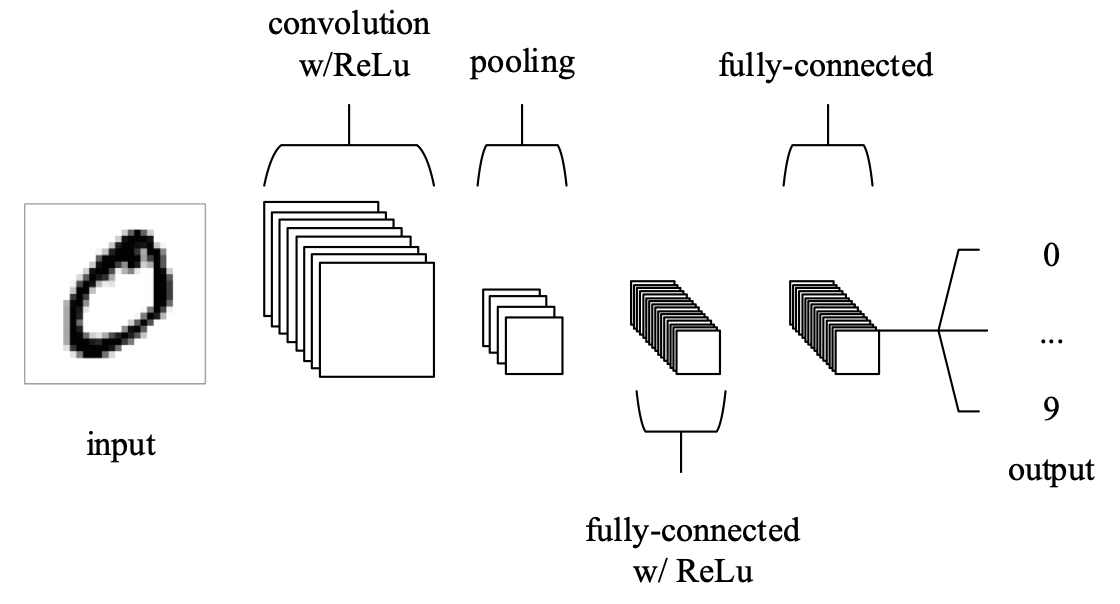
\includegraphics[width=0.8\linewidth]{images/CNN.png}
    \caption[Example of a Convolutional Neural Network architecture.]{Example of a Convolutional Neural Network architecture, designed to classify hand-written digits from the MNIST dataset \citep{OSheaNash2015}.}
    \label{fig:CNN}
\end{figure}

As network depth increases, CNNs learn progressively more abstract representations. Early layers capture low-level features such as edges and corners, while deeper layers encode higher-level semantic concepts such as object parts and complete object categories \citep{Krizhevsky2012}. This hierarchical feature learning is well suited to traffic scene analysis, where the model must simultaneously distinguish between visually similar object classes, including cars, heavy vehicles, cyclists, and pedestrians, under varying lighting conditions, viewpoints, and degrees of occlusion.

\subsection{Object Detection Architectures}
\label{sec:object_detection}

Object detection is a core computer vision task that integrates image classification, identifying the category of an object, with spatial localisation, determining its position within the image through bounding box regression \citep{Zhao2019}. For traffic monitoring applications, this dual capability is essential: detected road users must be assigned precise spatial positions to enable downstream trajectory estimation and traffic flow analysis.

Deep learning object detection models are commonly categorised into two paradigms based on their localisation strategy: two-stage and one-stage detectors.

\subsubsection{Two-Stage Object Detection}

Two-stage detectors decompose the detection task into sequential steps: region proposal generation followed by per-region classification and bounding box refinement \citep{Girshick2014, Ren2015}. Candidate object regions are first generated by a Region Proposal Network (RPN), and subsequently refined in a second stage. This design yields high localisation accuracy and strong performance on small or partially occluded objects, at the cost of increased computational complexity and reduced inference speed \citep{Zhao2019}. Extensions such as Mask R-CNN further augment this paradigm with instance-level segmentation capabilities \citep{He2017}, broadening the range of spatial analysis tasks that can be performed. However, the multi-stage pipeline renders two-stage detectors generally unsuitable for applications requiring continuous high-throughput video processing.

\subsubsection{One-Stage Object Detection}

One-stage detectors formulate detection as a single unified regression and classification problem, performing bounding box prediction and object categorisation simultaneously across the image in a single forward pass \citep{Redmon2016, Liu2016}. The elimination of the region proposal stage results in substantially lower inference latency and higher processing throughput, making one-stage architectures well suited for real-time video analysis. Early one-stage models exhibited reduced localisation accuracy relative to two-stage approaches, particularly for small or densely clustered objects \citep{Zhao2019}. However, successive architectural advances, including feature pyramid networks, anchor-free regression heads, and attention mechanisms, have substantially narrowed this performance gap \citep{Bochkovskiy2020}, making modern one-stage detectors competitive with two-stage models across standard detection benchmarks.

\subsubsection{Comparative Summary}

\begin{table}[H]
\centering
\begin{tabular}{p{3.5cm} p{5cm} p{5cm}}
\toprule
\textbf{Aspect} & \textbf{Two-stage detectors} & \textbf{One-stage detectors} \\
\midrule
Detection strategy & Region proposals + classification & Direct detection (single stage) \\
\addlinespace
Pipeline complexity & High & Moderate \\
\addlinespace
Inference speed & Slow & Fast (real-time capable) \\
\addlinespace
Detection accuracy & Very high & High (improving) \\
\addlinespace
Small object handling & Strong & Moderate to strong \\
\addlinespace
Computational cost & High & Lower \\
\addlinespace
Real-time suitability & Limited & Well suited \\
\addlinespace
Representative models & Faster R-CNN, Mask R-CNN & YOLO, SSD, RetinaNet \\
\bottomrule
\end{tabular}
\caption[Comparison of one-stage and two-stage object detection paradigms]{Comparison of one-stage and two-stage object detection paradigms \citep{Ma2024}.}
\label{tab:one_vs_two_stage}
\end{table}

As summarised in \autoref{tab:one_vs_two_stage}, one-stage detectors offer a more favourable trade-off between detection accuracy and computational efficiency for real-time traffic monitoring applications. Given the requirement for continuous video processing at practical frame rates and the need for downstream multi-object tracking, one-stage architectures represent the appropriate methodological basis for the detection pipeline developed in this thesis.

\subsection{YOLO-Based Object Detection}
\label{sec:yolo_models}

The You Only Look Once (YOLO) family of models represents the most widely 
adopted class of one-stage object detectors. YOLO models perform object 
localisation and classification in a single forward pass of a convolutional 
neural network, directly predicting bounding box coordinates and class 
probabilities across the full image without an intermediate region proposal 
stage \citep{Redmon2016}. A defining characteristic of the framework is its 
emphasis on global image reasoning: rather than processing candidate regions 
independently, YOLO considers the full image context during detection, which 
contributes to both fast inference and reduced false positives in visually 
complex scenes. This design enables end-to-end training and real-time 
inference, making YOLO-based models particularly well suited for continuous 
video processing applications.

Since its introduction in 2016, the YOLO family has undergone continuous 
architectural development, as illustrated in \autoref{fig:yolo_timeline}, 
with the most recent model in the Ultralytics ecosystem being YOLO26, 
released in 2025 \citep{Sapkota2025YOLOReview}. Key advances include the 
introduction of anchor boxes to improve localisation stability (YOLOv2), 
multi-scale feature prediction to enable detection across a range of object 
sizes (YOLOv3), and improved feature aggregation and training strategies to 
strengthen the speed-accuracy trade-off (YOLOv4) \citep{Sapkota2025YOLOReview}. 
Later generations introduced anchor-free detection heads and decoupled 
classification and regression branches (YOLOv8), as well as end-to-end 
optimisation with reduced post-processing overhead in more recent variants 
\citep{Sapkota2025YOLOReview}. Collectively, these developments reflect a 
consistent progression toward improved multi-scale detection, greater 
generalisation, and more flexible deployment across a range of hardware 
configurations.



\begin{figure}[H]
    \centering
    
\includegraphics[width=0.95\linewidth]{project/images/YOLO_timeline.png}
    \caption[Timeline of YOLO model releases, 2015--2025]{Timeline of YOLO 
    model releases, 2015--2025, including YOLO26 as the most recent 
    Ultralytics release. Source: \citep{DecadeOfYOLO, YOLOv1-v8, 
    Sapkota2025YOLOReview}.}
    \label{fig:yolo_timeline}
\end{figure}

For traffic monitoring at intersections, the properties of YOLO-based models 
align closely with the operational requirements of the application. Real-time 
inference at practical frame rates is necessary for continuous video 
processing, while robustness to varying illumination, partial occlusion, and 
background clutter is critical in uncontrolled outdoor environments. The 
multi-scale detection capability of modern YOLO variants enables simultaneous 
detection of objects across a range of sizes and distances within a single 
camera frame, which is essential when monitoring intersections where vehicles 
of varying dimensions, cyclists, and pedestrians must all be reliably 
identified. These characteristics make YOLO-based architectures a well-founded 
methodological basis for the detection pipeline developed in this thesis, as 
discussed further in \autoref{sec:methodology}.

\subsection{Multi-Object Tracking and Trajectory Extraction}
\label{sec:multi_object_tracking}
Measuring traffic parameters such as turning movements requires more than object detection alone; it necessitates Multi-Object Tracking. Multi-Object Tracking assigns a persistent and unique identifier to each detected road user across consecutive video frames, enabling trajectory estimation and movement analysis \citep{Hassan2024}.

Detection-Based Tracking is the most widely used Multi-Object Tracking paradigm in practical systems \citep{yang2022videoobjecttrackingbased}. Frameworks such as DeepSORT combine high-performance object detection with appearance-based association and motion prediction, typically using a Kalman filter. As Detection-Based Tracking relies directly on the quality and consistency of object detections, its performance is strongly influenced by the underlying detection model. This approach enables robust tracking even under temporary occlusion and is therefore well suited for traffic monitoring scenarios.

The resulting trajectory data enable the extraction of traffic volume, modal split, and turning movement information required for capacity and intersection analysis.


\section{Literature Review and Research Gap}
\label{sec:literature_review_research_gap}

This section reviews prior studies on deep learning–based vehicle detection for traffic monitoring, focusing on detection performance, computational efficiency, and real-world applicability. Identified limitations in existing work form the basis for the research gap addressed in this thesis.

\subsection{Deep Learning Approaches to Vehicle Detection}
\label{previous_work}
Several studies have investigated the performance of deep learning models for vehicle detection and classification using established benchmark datasets. For example, \cite{Ma2024} evaluated multiple one-stage and two-stage detection models on the PASCAL VOC 2012 dataset, a commonly used dataset in Computer Vision \citep{Everingham10,HuggingFacePascalVOC}. Although the dataset consists of still images rather than video sequences, the authors report that some one-stage models achieve processing speeds of up to 45 frames per second, but with lower detection accuracy compared to slower two-stage models. The study primarily formulates vehicle detection as a generic object detection task, and the number of vehicle classes used for classification is not explicitly specified.

\cite{Song2019VisionBasedVehicle} trained and evaluated a vision-based vehicle detection and counting system using YOLOv3 for object detection in combination with Oriented FAST and Rotated BRIEF (ORB), a feature detection and description algorithm, for multi-object tracking (MOT). The ORB algorithm extracts features within each detected bounding box and matches them across consecutive frames to maintain object correspondence over time \cite{Song2019VisionBasedVehicle}. The dataset consisted of images captured from a variety of viewpoints and included three vehicle classes: cars, buses, and trucks. The authors report a mean average precision (mAP) of 87.88\%, with very small class deviations from this value. Using ORB-based tracking, the system achieved a vehicle counting accuracy of 93.2\% and a direction recognition accuracy of 92.3\%, while maintaining processing speeds close to real time. Although these results demonstrate strong performance for traffic monitoring, the study is limited to highway environments and a small number of vehicle classes.

\cite{smartcities6050134} performed a large-scale comparison of Single Shot Detector (SSD), Faster R-CNN, and multiple YOLO variants using video data from 9 different datasets, recorded under diverse conditions, including nighttime, adverse weather, occlusions, and varying camera viewpoints . Their results show that YOLO-based models consistently outperform SSD (Single Shot Multibox Detector) and Faster R-CNN in terms of detection accuracy, localization precision, and computational efficiency. In particular, YOLO variants achieved detection accuracies above 95\% and overall classification accuracies exceeding 90\% for cars, trucks, and buses, while maintaining near real-time inference speeds. Although Faster R-CNN demonstrated competitive performance in some localization tasks, its substantially higher computational cost limited its suitability for continuous video-based traffic surveillance. The study therefore concludes that YOLO-based architectures provide the most favorable trade-off between accuracy and efficiency for real-time traffic monitoring applications.

\cite{YOLO-PEL} propose YOLOv8-PEL, a lightweight vehicle detection model built upon YOLOv8n, the smallest variant in the YOLOv8 family. The authors introduce architectural modifications aimed at improving multi-scale feature extraction and feature fusion, as well as a revised bounding box regression loss function to enhance localization stability. These changes reduce the number of model parameters and computational cost by approximately 25–30\% compared to the baseline YOLOv8n, while maintaining nearly identical mean average precision (mAP). The results demonstrate that lightweight architectural modifications can significantly improve real-time suitability without substantial loss in detection accuracy.

% unødvendig å ha med denne ?
%A comprehensive literature review by \citep{DeepLearningTrafficScene2025} shows that two-stage detectors such as Faster R-CNN and Mask R-CNN achieve high localization accuracy and perform well in complex scenes with occlusions, but their multi-stage pipelines and high computational demands limit their suitability for real-time deployment. In contrast, YOLO-based architectures are considered more suitable for real-time applications due to their single-pass design and favorable speed–accuracy trade-off. Nevertheless, the review reports that YOLO-based models remain challenged by small-object detection, densely overlapping road users, and adverse environmental conditions such as poor lighting and weather variability.



\subsection{Knowledge Gaps and Steps for Further Research}
\label{sec:research_gap}
\cite{Maity2022LastDecadeVehicleDetection} present a comprehensive survey of machine learning and deep learning–based approaches for automatic vehicle detection (AVD) and classification published over the last decade. Based on their review, the authors identify several research gaps. First, many AVD studies consider only a limited number of vehicle classes, highlighting the need to include a broader range of road users to better reflect real-world traffic diversity. Second, existing approaches often fail to explicitly evaluate robustness under occlusion and dense traffic conditions, despite these being common in operational environments.


Furthermore, \cite{DeepLearningTrafficScene2025} emphasize that YOLO-based detectors still require improvements in small-object and multi-scale detection, as well as increased robustness under adverse environmental conditions such as challenging lighting and weather. In addition, \cite{YOLO-PEL} argue that future research should prioritize practical validation of deep learning–based traffic monitoring systems in real-world deployment settings to assess their operational reliability and applicability.

To address these identified gaps, this thesis applies a deep learning–based object detection framework to video data from fixed roadside cameras in real intersection environments. The study expands beyond standard benchmark evaluations by focusing on a broader range of traffic participants relevant to Norwegian design guidelines. Furthermore, detection performance is evaluated under realistic operational conditions, including varying lighting, traffic density, and partial occlusion.

The extent to which the research gap is addressed is measured through a quantitative comparison between automatically extracted traffic parameters and manually conducted traffic counts. Specifically, traffic volumes, vehicle composition, and turning movements are compared using accuracy metrics and error analysis to determine whether the deep learning–based approach provides data of sufficient precision and reliability to serve as decision-support input in accordance with N100 and V121. This evaluation framework enables a systematic assessment of both detection performance and practical applicability in real-world intersection monitoring.

% Enda mer målbart: Inkludere flere klasser uten at det går på bekostning av accuracy
\chapter{Methods}
\label{chap:methods}

This chapter describes the methodology used to develop and evaluate the proposed vehicle detection and tracking pipeline, summarized in \autoref{fig:tech_workflow}. Video streams were collected from two SVV traffic camera stations across multiple times of day and weather conditions. A diverse set of frames was extracted and semi-automatically annotated, then partitioned into training, validation, and test splits before fine-tuning YOLO26n and YOLO26m. The trained detectors were subsequently combined with multiple MOT configurations, including ByteTrack, standard BoT-SORT, and two custom BoT-SORT variants optimized for daytime and nighttime conditions, and evaluated using a zone-based Origin--Destination framework on manually annotated clips. A dedicated day--night transition sequence was additionally used to demonstrate continuous operation under changing illumination.

\begin{figure}[H]
    \centering
    \includegraphics[width=1\linewidth]{project//images/tech_workflow4.png}
    \caption[Overall technical workflow of the custom vehicle detection and tracking pipeline]{Overall technical workflow of the custom vehicle detection and tracking pipeline developed in this thesis.}
    \label{fig:tech_workflow}
\end{figure}


\section{Data Description and Dataset Preparation}
This section describes the data source and acquisition process, summarizes data quality constraints, and details the annotation workflow and dataset partitioning used for model development and evaluation.

\subsection{Data Source and Acquisition}
The Norwegian Public Roads Administration operates 783 publicly accessible traffic camera stations across Norway. However, the majority of these stations provide only still images captured at ten-minute intervals and do not record continuous video streams. Among the limited number of stations that offer live video feeds, only a small subset is situated in intersections.

Two relevant camera stations were identified, with the first being mounted at Fv587 Haukeland, Bergen (Direction Arna), which is shown in \autoref{fig:haukeland_bilde}. The intersection is an unsignalized T-intersection, where a secondary road connects to the main road. Marked pedestrian crossings are present across the main approaches, and a bus bay with a sheltered stop is located along both roadsides. The area around the intersection includes a small number of residential buildings, open land, and roadside vegetation.

The second relevant camera station is mounted at Rv36 Kjørbekk (direction Porsgrunn), which is shown in \autoref{fig:kjørbekk_bilde}. The intersection is also an unsignalized T-intersection where a secondary road connects to the main road. Towards the top of the frame, the main road leads into a roundabout that facilitates traffic distribution in various directions. A pedestrian and bicycle path runs parallel to the main road on the right side. Near the T-intersection, an underground pedestrian crossing allows individuals to safely cross beneath the main road. Additionally, a bus stop is located along the roadside on the left.

\begin{figure}[H]
     \centering
     \begin{subfigure}[b]{0.48\textwidth}
         \centering
         
\includegraphics[width=\linewidth]{project/images/haukeland_bilde.png}
         \caption{Fv587 Haukeland}
         \label{fig:haukeland_bilde}
     \end{subfigure}
     \hfill
     \begin{subfigure}[b]{0.48\textwidth}
         \centering
         
\includegraphics[width=\linewidth]{project/images/kjørbekk_bilde.jpg}
         \caption{Rv36 Kjørbekk}
         \label{fig:kjørbekk_bilde}
     \end{subfigure}
     \caption{Snapshots of video streams at different camera stations. Source: \cite{SVV_HaukelandKamera}}
     \label{fig:combined_cameras}
\end{figure}

The video data was captured from the SVV live streams using an FFmpeg script targeting the m3u8-stream URLs (Appendix~\ref{app:ffmpeg}). To manage the data efficiently, the continuous streams were segmented into five-minute MPEG-4 video clips. Rather than using the entire raw video duration, a strategic sampling approach was implemented to maximize the quality and relevance of the dataset.

Initially, frames were extracted at random intervals to establish a baseline. However, as the base YOLO26 model is pre-trained on the COCO dataset, it already possessed high proficiency in identifying standard passenger cars. To focus the training on specialized vehicle classes, the strategy shifted toward manual frame extraction, specifically targeting intervals containing heavy vehicles.

As the custom model’s weights were updated and its performance improved, a more automated model-in-the-loop approach was introduced. A custom script was developed to process the video segments, running the current YOLO weights on every frame and automatically extracting only those images where the model detected heavy vehicles. This filtering process significantly reduced the redundancy of the dataset, ensuring that the manual annotation effort was concentrated on the most informative samples for the model's specific objectives. This process resulted in a final dataset of 1282 images.


\subsection{Data Quality and Limitations}

The video data varies in resolution and frame rates between the two recording sites. The stream from Fv587 Haukeland is captured at a resolution of 800 × 450 pixels. During the data collection period, this stream was delivered at approximately 10 FPS (7 FPS at night) and contained a large grey censoring box in the upper right corner. As of April 13$^{th}$ 2026, the grey box has been removed, the frame rate has been doubled, and the field of view has been slightly zoomed out. The Rv36 Kjørbekk station provides a higher spatial resolution of 1024 × 576 pixels, but at a lower frame rate of roughly 5 FPS. To ensure the model's robustness and ability to generalize, the dataset was extracted at various times of the day, encompassing a wide range of weather conditions, from clear daylight to dark, foggy, and snowy environments, as illustrated in \autoref{fig:weather_conditions}. This diversity in the training data is crucial for the model to accurately identify vehicles despite shifting shadows, varying light intensity, and reduced visibility due to precipitation.

\begin{figure}[H]
    \centering
    
\includegraphics[width=1\linewidth]{project/images/weather_conditions.png}
    \caption[Examples of environmental and lighting variations in the dataset]{Examples of environmental and lighting variations in the dataset. Source: \cite{SVV_HaukelandKamera}}
    \label{fig:weather_conditions}
\end{figure}

The data acquisition process was subject to several constraints that shaped the final composition of the dataset. Since SVV does not provide access to historical video archives, the study relied exclusively on live-stream captures. This prevented the retrieval of data from different seasons or specific past traffic events, effectively tying the dataset to the environmental conditions present during the recording period. Consequently, because the recordings were conducted during the Norwegian winter/early spring, the dataset reflects a notable scarcity of pedestrians, cyclists, and motorcyclists. Furthermore, the relatively low traffic volume at the selected sites necessitated extended recording periods to ensure a sufficient number of observations for the less frequent vehicle classes.

A significant technical limitation is the automated privacy masking implemented by SVV on their public live streams. To comply with privacy regulations, the system is designed to blur or pixelate license plates and faces. In practice, this masking introduces image artifacts and removes fine-grained texture information, which can reduce classification reliability for visually similar vehicle categories. Moreover, because the masking can change abruptly between frames, it can degrade appearance-based association in multi-object tracking and increase the risk of ID switches. In many instances, particularly at the Rv36 Kjørbekk station, this automated censorship is overly aggressive, occasionally causing the entire vehicle to become heavily pixelated. This loss of visual data poses a challenge for both manual annotation and model training.

This technical challenge is further compounded by the subjective nature of manual classification. As the annotators are not professional vehicle experts, certain edge cases proved difficult to categorize with absolute certainty. Visual ambiguity, often made worse by distance, poor weather conditions or pixelation, introduces a margin of human error in the labeling process. These inconsistencies in the ground-truth data may impact the model’s ability to learn the fine-grained distinctions required to accurately differentiate between visually similar vehicle configurations.


\subsection{Data Annotation}
\label{sec:data_annotation}
To address the research gap identified in Section~\ref{sec:research_gap}, where most existing automatic vehicle detection studies are limited to a small number of standard vehicle classes and fail to capture the full diversity of real-world road users \citep{Maity2022LastDecadeVehicleDetection}, the development of the custom object detection model follows an iterative, semi-automated annotation pipeline specifically designed to incorporate a broader and more granular set of vehicle classes.

As shown in \autoref{fig:annotation_workflow}, the process begins by defining the target vehicle classes, followed by an initial pre-annotation phase. To ensure a consistent and reproducible labeling environment, Label Studio was deployed using Docker, allowing for seamless integration of the annotation interface with custom backend scripts. A subset of images is initially processed using a base YOLOv8 model to generate preliminary labels. These are then manually reviewed within Label Studio to adjust bounding boxes, correct misclassifications, and incorporate ``non-COCO'' classes, such as \textit{light truck}, \textit{heavy truck}, and \textit{semi-trailer / combination vehicle}. Once a high-quality initial dataset is established, it is used to train a custom model. This trained model is subsequently deployed to pre-annotate new image batches, after which human annotators perform final manual corrections. This approach ensures high ground-truth accuracy while significantly reducing the time required to expand the dataset.

\begin{figure}[H]
    \centering
    \includegraphics[width=1\linewidth]{project/images/annotation-workflow.png}
    \caption{Annotation workflow diagram.}
    \label{fig:annotation_workflow}
\end{figure}

\subsubsection*{Annotation Rules and Class Definitions}
To ensure consistency and reduce ambiguity, vehicles were categorized based on physical characteristics and axle counts. Objects at extreme distances or those with insufficient visibility were excluded from the dataset to prevent the model from learning from ambiguous features. \autoref{fig:classes} visualizes the classes that are described below.

\begin{itemize}
    \item \textbf{Car}: Includes all standard passenger vehicles, including sedans, SUVs, and commercial vans.
    \item \textbf{Bus}: Includes public transit buses and other buses.
    \item \textbf{Light Truck}: Two-axle commercial and delivery vehicles, including passenger cars towing small trailers, whose length and weight profiles are more consistent with light freight vehicles than private cars. Tractors and camping vans are also included in this category.
    \item \textbf{Heavy Truck}: Rigid trucks with three axles. In addition, Semi-trailer tractor units (bobtails) traveling without a trailer are included.
    \item \textbf{Semi-trailer / Combination Vehicle}: Includes all articulated vehicles with four or more axles.
    \item \textbf{Motorcycle}: Includes both high-capacity motorcycles and small-engine scooters.
    \item \textbf{Bicycle}: Includes all human-powered or electric bicycles.
    \item \textbf{Person}: Includes individual pedestrians and stationary persons within the traffic environment.
\end{itemize}

\begin{figure}[H]
    \centering
    
\includegraphics[width=0.8\linewidth]{project//images/classes.png}
    \caption{Visualization of the 8 classes in the dataset.}
    \label{fig:classes}
\end{figure}

\subsection{Dataset Partitioning}
Scikit-learn was used to partition the 1282 annotated images using a randomized 70/15/15 split into training, validation, and test subsets (\autoref{fig:tvt_split}). The training set was used to optimize model weights, while the validation set was used to monitor generalization during training, apply early stopping, and select the best-performing checkpoint. The test set was held out throughout training and was used only once for the final evaluation of the selected model, providing an unbiased estimate of performance on unseen data.

\begin{figure}[H]
    \centering
    \includegraphics[width=0.75\linewidth]{project//images/tvt_split.png}
    \caption{Train/Validation/Test Split}
    \label{fig:tvt_split}
\end{figure}


\section{Model Selection}
Following the theoretical evaluation of modern object detection architectures in \autoref{sec:computer_vision}, YOLO26 was selected as the core framework for this study. Based on the performance metrics summarized in \autoref{tab:yolo26-sizes}, this study evaluates two specific versions of the YOLO26 architecture to address the trade-off between computational efficiency and detection precision.

\begin{itemize}
   \item \textbf{YOLO26n (Nano):} Selected for its high CPU efficiency, achieving 26\,FPS (ONNX Runtime) on standard hardware. To evaluate practical feasibility, YOLO26n is therefore paired with the most lightweight tracker configuration and benchmarked end-to-end on CPU for the complete pipeline.

   \item \textbf{YOLO26m (Medium):} Chosen as the high-performance benchmark. The large (l) and extra-large (x) variants were excluded due to higher computational demands with diminishing returns relative to YOLO26m for our deployment-oriented setting.
\end{itemize}

\begin{table}[H]
\centering
\small
\caption[Ultralytics YOLO26 detection performance metrics on COCO val2017]
{Ultralytics YOLO26 detection performance metrics on COCO val2017. Adapted from \cite{sapkota2026yolo26keyarchitecturalenhancements}.}
\label{tab:yolo26-sizes}
\begin{tabular}{@{}lrrrrrr@{}}
\toprule
Model & \makecell{mAP$^{50-95}$ \\ (e2e)} & \makecell{Speed CPU \\ ONNX (ms)} & \makecell{Speed T4 \\ TRT10 (ms)} & \makecell{FPS CPU \\ (approx.)} & \makecell{FPS T4 \\ (approx.)} & \makecell{Params \\ (M)} \\
\midrule
YOLO26n & 40.1 & 38.9 & 1.7 & 26 & 588 & 2.4 \\
YOLO26s & 47.8 & 87.2 & 2.5 & 11 & 400 & 9.5 \\
YOLO26m & 52.5 & 220.0 & 4.7 & 4.5 & 213 & 20.4 \\
YOLO26l & 54.4 & 286.2 & 6.2 & 3.5 & 161 & 24.8 \\
YOLO26x & 56.9 & 525.8 & 11.8 & 1.9 & 85 & 55.7 \\
\bottomrule
\end{tabular}
\end{table}

\subsection{Training Configuration and Hyperparameters}
The selected YOLO26n and YOLO26m models were fine-tuned in Google Colaboratory using an NVIDIA Tesla T4 GPU and Python 3.12.12. The detection architecture was implemented via the Ultralytics (v8.3.0) framework.

Each model was trained for 100 epochs using an input image size of 640 pixels and a batch size of 16. To optimize training efficiency and prevent overfitting, an early-stopping patience of 20 epochs was implemented, which terminates the process if no improvement is detected in the validation metrics. The model’s weights are initialized from COCO-pretrained checkpoints.

The training of the model was conducted using the default hyperparameter configurations provided by the YOLO26 framework (Appendix~\ref{app:hyperparameters}). Traditionally, achieving optimal performance in object detection requires iterative "tuning sessions," where the model is retrained multiple times to find the best combination of variables. In this study, no manual hyperparameter tuning was performed, as this process is both time-consuming and computationally expensive, particularly under the resource constraints of a Google Colab Tesla T4 GPU environment. The default training configuration also includes data augmentation techniques, such as mosaic augmentation, HSV color jitter and horizontal flipping. To improve reproducibility across runs, the random seed was fixed to 42, ensuring consistent stochastic behavior. 

Additionally, the architectural advancements in YOLO26 significantly mitigate the necessity for such extensive tuning. By utilizing an NMS-free design, the requirement to manually optimize IoU and confidence thresholds is entirely removed. Furthermore, the implementation of the MuSGD optimizer provides a more robust and stable learning process than the SGD or AdamW optimizers used in models ranging from YOLOv8 to YOLOv11, which required extensive hyperparameter tuning \citep{sapkota2026yolo26keyarchitecturalenhancements}.

\section{Multi-Object Tracking for Origin-Destination Estimation}
\label{sec:method_tracking_od}

After fine-tuning YOLO26 on the SVV intersection dataset, the resulting custom-trained YOLO26n and YOLO26m models are used as the detection backbone in the full video-processing pipeline. While object detection provides per-frame bounding boxes and vehicle class predictions, the extraction of traffic engineering parameters such as turning movements requires consistent vehicle identities over time. Therefore, multi-object tracking is applied to associate detections across consecutive frames and reconstruct vehicle trajectories through the intersection.

Building on these trajectories, an origin--destination (O--D) estimation procedure is implemented to assign each tracked vehicle an entry approach (origin) and an exit approach (destination) based on predefined spatial gate regions. This enables automated estimation of turning movements and directional traffic volumes, which are later compared against manual ground-truth counts for validation.

\subsection{Tracking Algorithm}
\label{sec:method_tracker}

Multi-object tracking is performed using the tracking algorithms available in the Ultralytics YOLO framework. The implementation evaluates these different trackers: ByteTrack, standard BoT-SORT, and two custom BoT-SORT configurations optimized for daytime and nighttime conditions, respectively.

All trackers are applied in track mode with persistent identities enabled, allowing each detected vehicle to be assigned a consistent track ID across frames. ByteTrack serves as a lightweight baseline for performance comparison, while BoT-SORT is employed for its ability to incorporate appearance-based re-identification (ReID). However, the production pipeline employs an adaptive approach: a custom BoT-SORT configuration is selected dynamically based on detected lighting conditions, as detailed in Section~\ref{sec:method_dynamic_switching}.

In addition to the default implementations, custom BoT-SORT configurations are deployed to improve tracking robustness in traffic scenarios. For daytime operations, the configuration is specified in \textit{day\_botsort.yaml}. For night-time operations, a conservative configuration file \textit{night\_botsort\_conservative.yaml} is used to handle low-light conditions and headlight-induced artifacts while minimizing false track associations. 

Table~\ref{tab:botsort-config} summarizes the parameters used in both configurations. Compared with daytime settings, the conservative night profile uses stricter association criteria and a substantially larger track buffer to reduce ID fragmentation and false associations in low-light scenes. Appearance-based ReID is enabled in the daytime configuration to leverage visual cues for re-association, but disabled at night where those cues are less reliable.

\begin{table}[H]
\centering
\small
\setlength{\tabcolsep}{8pt}
\renewcommand{\arraystretch}{1.15}
\caption[Custom BoT-SORT configuration parameters]{Comparison of custom BoT-SORT configurations used in daytime and night-time experiments.}
\begin{tabular}{@{}lcc@{}}
\textbf{Parameter} & \textbf{Day BoT-SORT} & \textbf{Night BoT-SORT (Conservative)} \\
\midrule
\texttt{track\_high\_thresh}  & 0.25             & 0.28 \\
\texttt{track\_low\_thresh}   & 0.10             & 0.12 \\
\texttt{new\_track\_thresh}   & 0.35             & 0.28 \\
\texttt{track\_buffer}        & 30               & 90 \\
\texttt{match\_thresh}        & 0.75             & 0.90 \\
\texttt{fuse\_score}          & True             & True \\
\texttt{gmc\_method}          & \texttt{none}    & \texttt{none} \\
\texttt{proximity\_thresh}    & 0.50             & 0.75 \\
\texttt{appearance\_thresh}   & 0.25             & 0.35 \\
\texttt{with\_reid}           & True             & False \\
\texttt{model}                & \texttt{auto}    & \texttt{auto} \\
\bottomrule
\end{tabular}
\label{tab:botsort-config}
\end{table}

In brief, \texttt{track\_high\_thresh} and \texttt{track\_low\_thresh} control which detections are used for association, \texttt{new\_track\_thresh} sets the confidence required to start a new track, and \texttt{track\_buffer} determines how long a lost track is kept alive. The matching thresholds \texttt{match\_thresh}, \texttt{proximity\_thresh}, and \texttt{appearance\_thresh} control how strict association is in motion and appearance space, while \texttt{with\_reid} enables appearance-based re-identification and \texttt{gmc\_method} specifies global motion compensation.


Detection-to-track association is controlled through the confidence and IoU thresholds in the YOLO tracking pipeline. These parameters are tuned to balance detection sensitivity and tracking stability. The different tracker configurations are evaluated against ground-truth origin--destination counts, and the best-performing setup is selected for further analysis.


\subsection{Gate-Zone Definition and Calibration}
\label{sec:method_zones}

To enable traffic flow analysis, spatial gate zones are manually defined as polygons in image coordinates $(x,y)$, where $x$ increases to the right and $y$ increases downwards. Each polygon corresponds to a directional entry or exit (e.g., North, South, East) or a detection region for pedestrians. Zones are assigned a type indicator: \textit{vehicle} for vehicle O--D counting or \textit{person} for pedestrian detection.

The zones are intentionally drawn slightly larger than the visible roadway to increase robustness against detection noise, small localization errors, and partial occlusions. A visualization step overlays the polygons on a reference frame together with a coordinate grid, allowing efficient and precise placement of polygon vertices. This facilitates manual calibration of the zones by making it easier to read off coordinates directly from the image.

\textbf{Vehicle zones:} Used for origin--destination (O--D) counting via the logic described in Section~\ref{sec:method_od_logic}.

\textbf{Person zones:} Used for pedestrian counting based on dwell time. A pedestrian is counted if a person-class detection (identified by class label) resides in the zone for a threshold number of frames (default: 10 frames). This approach avoids double-counting pedestrians who linger at a location.

An example of the defined gate zones and the coordinate grid used during calibration is shown in Figure~\ref{fig:Gatezones}. Each zone is assigned a semantic label, which is used directly in the O--D computation and person counting.

\begin{figure}[H]
    \centering
    
\includegraphics[width=0.9\linewidth]{project/images/Gatezones.png}
    \caption{Visualization of manually defined gate zones overlaid on a reference frame, including a coordinate grid used for calibration.}
    \label{fig:Gatezones}
\end{figure}

\subsection{Tracking Pipeline}
\label{sec:method_pipeline}

The full processing pipeline is implemented in the function \texttt{run\_video\_deploy}, which converts raw video into O--D outputs through the following steps as visualized in \autoref{fig:flow_tracking}:

\begin{figure}[H]
    \centering
    \includegraphics[width=1.0\linewidth]{project/images/flow_tracking.png}
    \caption{Tracking Pipeline}
    \label{fig:flow_tracking}
\end{figure}

\subsubsection{Video processing and ROI selection}
The input video is read using OpenCV, and metadata such as resolution, frame rate, and total frames are extracted. To reduce computational cost and avoid edge artifacts, tracking is performed only within a central region of interest (ROI), defined by horizontal and vertical ratios $(r_w, r_h)$. 

In addition, restricting the analysis to the central region improves classification reliability, as objects near the image boundaries are more prone to partial visibility, perspective distortion, and truncated bounding boxes, which can negatively affect both detection and classification performance.
\[
x_0=\left\lfloor\frac{(1-r_w)W}{2}\right\rfloor,\quad x_1=W-x_0,\quad
y_0=\left\lfloor\frac{(1-r_h)H}{2}\right\rfloor,\quad y_1=H-y_0.
\]
Each frame is cropped to this ROI prior to inference, while the ROI boundary is visualized in the output video.

\subsubsection{Dynamic Tracker Switching}
\label{sec:method_dynamic_switching}

To maintain robust tracking across varying lighting conditions (day, night, and twilight), the pipeline employs adaptive tracker selection based on real-time illumination analysis. The system automatically detects the current lighting condition and selects an appropriate tracker configuration.

Mode detection is based on HSV color saturation. The mean saturation of each frame is compared to a threshold (\texttt{sat\_threshold = 20.0}), where frames with \texttt{sat\_mean < sat\_threshold} are classified as nighttime. In the SVV video streams, the transition from day to night occurs abruptly, with the footage switching from full color to near-grayscale, resulting in a sharp drop in saturation. To reduce sensitivity to short-term fluctuations, saturation values are averaged over a rolling window of approximately 2 seconds before thresholding.

Figure~\ref{fig:saturation_transition} illustrates the saturation signal during a transition sequence, showing how the detected drop aligns with the stream’s day–night switch and triggers a corresponding change in tracking configuration.



\begin{figure}[H]
    \centering
    \includegraphics[width=1\linewidth]{project/images/saturation.png}
    \caption{Rolling HSV saturation (\texttt{sat\_mean}) over time for the 10-minute transition video, including the decision threshold and detected tracker switch points.}
    \label{fig:saturation_transition}
\end{figure}

To prevent tracker flickering during twilight transitions or lighting artifacts, mode changes are subject to a persistence requirement. The system only commits to a new mode after it has been consistently detected for 5 seconds. This hysteresis mechanism prevents transient lighting fluctuations from triggering unnecessary tracker switches while still allowing adaptation to sustained illumination changes.

When a mode switch is detected, the tracker is switched from the best day configuration to the best night configuration (or vice versa). In practice, some identities can split across the switch; these split IDs are handled in a dedicated post-processing step during finalization, described in Section~\ref{sec:method_split_id_recovery}.

\subsubsection{Detection and tracking}
A YOLO-based detector is executed in tracking mode with persistent identities. The tracker assigns a unique ID to each vehicle and maintains this identity across frames, enabling trajectory reconstruction and temporal analysis.

Each detected bounding box $(x_1,y_1,x_2,y_2)$ is reduced to a single representative point. Two alternatives are supported: the centroid and the bottom-center point. The bottom-center point,
\[
\left(\frac{x_1+x_2}{2},\,y_2-\delta\right),
\]
is used by default, as it better approximates the vehicle's position on the road plane and is less sensitive to perspective distortion.

A vehicle is considered inside a gate zone if its tracking point lies within the corresponding polygon. This is evaluated using a standard point-in-polygon test.

\subsubsection{Zone Stabilization and O--D Logic}
\label{sec:method_od_logic}

To avoid spurious transitions caused by detection noise near zone boundaries, zone assignments are stabilized using a dwell-time constraint. For each track $i$, a short history buffer of recent zone assignments is maintained:
\[
H_t(i) = [z_{t-K+1}(i), \ldots, z_t(i)],
\]
where $z_t(i)$ denotes the zone at frame $t$. A stable zone is declared if the last $K$ non-null entries are identical. In this study, $K=3$ frames (the default \texttt{zone\_dwell\_frames} parameter) is used as a compromise between responsiveness and robustness. Additionally, only tracks that have been active for at least \texttt{min\_track\_frames} are eligible for O--D counting, filtering out spurious detections (typically 5 frames in daytime experiments, and reduced to 2 frames in selected night/transition evaluations).

The O--D logic is defined as follows:
\begin{itemize}
    \item The first stable zone observed for a track defines its origin $o(i)$.
    \item The destination $d(i)$ is taken as the last stable zone observed for that track before finalization.
    \item Each track contributes at most one O--D event $o(i) \rightarrow d(i)$.
\end{itemize}

An O--D event is counted only when $o(i) \neq d(i)$ at finalization (e.g., when the track is inactive for the configured gap), which ensures that each vehicle is counted once and reduces overcounting from short-term boundary oscillations.

\subsubsection{Track-Level Class Stabilization}
\label{sec:method_class_stabilization}

To obtain robust vehicle classification, class predictions are aggregated over the lifetime of each track. For each track ID, both the predicted classes and their associated confidence scores are stored across frames.

For each class, the number of occurrences and the average confidence are computed. A class is considered stable if it appears in at least five frames. If one or more stable classes exist, the class with the highest average confidence is selected. Otherwise, the class that appears most frequently is chosen.

This approach reduces the impact of occasional misclassifications and provides more consistent class labels for O--D analysis.

\subsubsection{O--D Matrix Construction}
\label{sec:method_od_matrix}

O--D counts are aggregated by destination $d$, origin $o$, and vehicle class $c$:
\[
M_{d,o,c} \leftarrow M_{d,o,c} + 1.
\]
In addition to the aggregated matrix, an event log is maintained containing the frame index, track ID, origin, destination, class label, and confidence for each detected transition.

\subsubsection{Split ID Recovery}
\label{sec:method_split_id_recovery}
During extended video analysis, a single vehicle track may become fragmented into multiple identities. This can happen when the tracker switches between day and night configurations, but also when detections are interrupted by brief occlusions, low confidence, or other tracking gaps. Such fragmentation results in incomplete O--D trajectories and can cause undercounting. To mitigate this effect, a post-processing step reconstructs fragmented identities during finalization by matching compatible track fragments. As mentioned as a knowledge gap, occlusion is a frequent cause of such fragmentation and identity switches in MOT systems, yet handling it explicitly remains an open challenge in vehicle-tracking research \citep{Hassan2024}.

Track fragments are extracted from the detection history, with each fragment defined by its temporal interval (start and end frame), spatial positions (start and end points), dominant vehicle class, and an estimated velocity vector. The recovery step considers two types of cases: tracks that already contain a valid origin--destination transition but were not counted earlier, and pairs of fragments that may belong to the same vehicle across a gap. Candidate matches are evaluated using a multi-criteria cost function that penalizes:
\begin{itemize}
    \item \textbf{Spatial distance:} Euclidean distance between the end position of the earlier fragment and the start position of the later fragment, compared against a threshold (default: $\text{max\_dist\_raw} = 180$ pixels).
    \item \textbf{Velocity-predicted distance:} For fragments with sufficient temporal support, the expected continuation point is estimated using the fragment velocity. The distance between the predicted and observed start positions is compared against a stricter threshold (default: $\text{max\_dist\_pred} = 160$ pixels).
    \item \textbf{Class consistency:} Fragments with different dominant vehicle classes incur a penalty (default: $\text{class\_penalty} = 40$ pixels equivalent) to the distance metric, reducing but not preventing matches between visually distinct classes.
    \item \textbf{Temporal proximity:} Only fragments separated by a temporal gap of less than the threshold (default: $\text{max\_gap\_seconds} = 3$ seconds) are considered for matching.
\end{itemize}
Matches are resolved greedily by selecting the lowest-cost candidate that satisfies all constraints. Successfully matched fragments are merged into a single identity, while valid single-fragment trips that were missed earlier are added directly to the O--D counts. This improves the completeness of the trajectory set and the accuracy of the final O--D matrix.

\subsubsection{Outputs and Quality Control}
\label{sec:method_outputs}
The pipeline produces compact, machine-readable outputs and brief QC artifacts:
\begin{itemize}
    \item \textbf{Exports:} annotated video (MP4), event logs, trajectories (CSV/JSON), and full track dumps (pickle/JSON).
    \item \textbf{Tracking statistics:} processing time, achieved FPS, total detections, frames without track IDs, and a split-id summary.
    \item \textbf{Evaluation exports:} O--D matrices and summary metrics (class error, route error, total error, \% error)
    \item \textbf{Reproducibility metadata:} model version, tracker configurations, time for tracker switching, random seed, and run timestamp are recorded with outputs.
\end{itemize}

An example of the annotated output is shown in Figure~\ref{fig:tracking_output}. The figure illustrates how detected vehicles are represented with bounding boxes, track IDs, and class labels, as well as their trajectories over time. The region of interest (ROI) is highlighted. In addition, live current origin-destination counts are displayed.

\begin{figure}[H]
    \centering
    
\includegraphics[width=0.9\linewidth]{project/images/tracking_output.png}
    \caption{Annotated tracking output showing detections, trajectories, gate zones, and O--D overlay.}
    \label{fig:tracking_output}
\end{figure}

\subsection{Experimental Design and Evaluation Protocol}
\label{sec:method_eval_protocol}

Tracking performance is evaluated end-to-end as a detection + tracking + zone-based origin--destination (O--D) aggregation pipeline. Two detectors (YOLO26n and YOLO26m) are combined with three tracking strategies, yielding six configurations per lighting condition: ByteTrack, default BoT-SORT, and a custom BoT-SORT profile tuned for the relevant time of day.

The evaluation follows a staged protocol:

\begin{enumerate}
    \item \textbf{Daytime screening (15 minutes):} six configurations are evaluated on a 15-minute daytime segment to compare detector capacity and tracker choice under normal lighting and to select the best-performing daytime setup.
    \item \textbf{Daytime validation (1 hour, rush-hour):} the selected best daytime configuration is evaluated on a 1-hour daytime rush-hour segment to assess performance stability over longer sequences.
    \item \textbf{Night-time evaluation (1 hour):} six configurations are evaluated on a 1-hour night-time segment. Night-time processing is faster due to the reduced frame rate of the video stream, making full comparison across configurations computationally feasible.
    \item \textbf{Day--night transition (10 minutes):} an additional twilight sequence is used to evaluate autonomous operation across changing lighting conditions, using dynamic switching between the day-optimized and night-optimized tracker configurations.
\end{enumerate}


%The proposed system is evaluated under four distinct experimental scenarios. First, all six model--tracker combinations are tested on a 15-minute daytime segment to assess baseline performance and compare configurations under controlled conditions. Second, the best-performing configuration from this stage is further evaluated on a 1-hour daytime rush-hour segment to assess temporal stability under increased traffic density.

%Third, all configurations are evaluated on a 1-hour night-time segment to assess robustness under low-light conditions. Finally, a 10-minute day--night transition sequence is used to evaluate system behavior under changing illumination, including the effectiveness of the dynamic tracker switching mechanism.
\chapter{Results}
\label{chap:results}

\section{YOLO Results}
\label{sec:training-results}
This section presents the performance of the YOLO26n and YOLO26m model for vehicle detection and classification, and provides the empirical basis for assessing the first research question. For YOLO26n, the training process was conducted for 87 epochs, at which point early stopping was triggered as the validation loss reached a plateau. YOLO26m finished all 100 epochs. The following results are evaluated based on both the validation dataset used during training and an independent test set to ensure the model's generalizability to unseen data. The train/val/test split is identical for both model sizes.

\subsection{Training and Validation}
\label{sec:yolo_train_val}
\subsubsection*{mAP$^{50-95}$ and mAP$^{50}$}
The training progress of the YOLO26n and YOLO26m models was evaluated using mAP$^{50-95}$ and mAP$^{50}$. As shown in \autoref{fig:train_val_map}, both models exhibit a consistent upward trajectory. The YOLO26m model achieves a higher peak mAP$^{50}$ of 0.9027, compared to 0.7421 for the YOLO26n variant. Similarly, for the stricter mAP$^{50-95}$ metric, YOLO26m reaches a peak of 0.7237, while YOLO26n peaks at 0.5989. Performance for both models effectively plateaus after epoch 55, indicating they have reached their learning capacity for the dataset.

\begin{figure}[H]
\centering

\includegraphics[width=1.0\linewidth]{project/images/yolo_n_vs_m/train_val_map.png}
\caption{Training progress comparison of YOLO26n and YOLO26m for mAP$^{50-95}$ (left) and mAP$^{50}$ (right).}
\label{fig:train_val_map}
\end{figure}

\subsubsection*{Precision and Recall}
The specific trade-offs between Precision and Recall are illustrated in \autoref{fig:train_val_pr}. While both metrics maintain a general upward trend, they exhibit higher volatility compared to the mAP scores. The YOLO26m variant demonstrates significantly superior sensitivity, reaching a peak recall of 0.8658, whereas YOLO26n reaches a maximum of 0.7085. In terms of Precision, YOLO26m peaks at 0.9239 and YOLO26n at 0.9083. Although Precision shows sharp fluctuations between epochs 10 and 50, both models stabilize in the later stages of training, ensuring reliable vehicle detection.

\begin{figure}[H]
\centering

\includegraphics[width=1.0\linewidth]{project/images/yolo_n_vs_m/train_val_pr.png}
\caption{Training progress comparison of YOLO26n and YOLO26m for Precision (left) and Recall (right).}
\label{fig:train_val_pr}
\end{figure}

For a more comprehensive overview of the model’s training and validation, validation set results are presented in Appendix \ref{app:raw_metrics}. 



\subsection{Performance on Test Set}
\label{sec:test_results}
The final performance of both the YOLO26n and YOLO26m models was evaluated on the same independent test set of 193 images containing 761 object instances, as detailed in \autoref{tab:test_results_n} and \autoref{tab:test_results_m}. The YOLO26n model achieved an overall mAP$^{50}$ of 0.693 and an mAP$^{50-95}$ of 0.556, while the YOLO26m variant delivered noticeably stronger results with an mAP$^{50}$ of 0.808 and an mAP$^{50-95}$ of 0.638. Notably, the validation metrics were even stronger.

Analysis of individual classes shows that the ’Car’ category remains the most accurately detected for both models, with AP$^{50}$ values of 0.945 (YOLO26n) and 0.960 (YOLO26m) and recall values above 0.91. Large vehicle categories such as ’Heavy Truck’ and ’Semi-trailer’ also demonstrated high reliability across both variants (mAP$^{50}$ of 0.743/0.817 and 0.869/0.912, respectively). Only two instances of bicycles ended up in the test set, and received a very low score, especially on the nano model.

\begin{table}[H]
\centering
\caption{YOLO26n Test Set Results ($n=193$)}
\label{tab:test_results_n}
\begin{tabular}{lcccccc}
\toprule
\textbf{Class} & \textbf{Images} & \textbf{Instances} & \textbf{Presicion} & \textbf{Recall} & \textbf{mAP$^{50}$} & \textbf{mAP$^{50-95}$} \\
\midrule
all & 193 & 761 & 0.605 & 0.750 & 0.693 & 0.556 \\
\midrule
bicycle & 2 & 2 & 0.307 & 0.500 & 0.188 & 0.118 \\
bus & 20 & 21 & 0.662 & 0.745 & 0.708 & 0.563 \\
car & 161 & 580 & 0.838 & 0.936 & 0.945 & 0.780 \\
heavy truck & 42 & 45 & 0.674 & 0.780 & 0.743 & 0.654 \\
light truck & 31 & 33 & 0.564 & 0.606 & 0.697 & 0.624 \\
motorcycle & 6 & 6 & 0.525 & 1.000 & 0.840 & 0.634 \\
person & 19 & 25 & 0.566 & 0.640 & 0.557 & 0.322 \\
semi-trailer & 48 & 49 & 0.705 & 0.796 & 0.869 & 0.756 \\ \hline
\end{tabular}
\end{table}

\begin{table}[h]
\centering
\caption{YOLO26m Test Set Results ($n=193$)}
\label{tab:test_results_m}
\begin{tabular}{lcccccc}
\toprule
\textbf{Class} & \textbf{Images} & \textbf{Instances} & \textbf{Presicion} & \textbf{Recall} & \textbf{mAP$^{50}$} & \textbf{mAP$^{50-95}$} \\
\midrule
all & 193 & 761 & 0.810 & 0.781 & 0.808 & 0.638 \\
\midrule
bicycle & 2 & 2 & 0.828 & 0.500 & 0.495 & 0.346 \\
bus & 20 & 21 & 0.806 & 0.793 & 0.828 & 0.690 \\
car & 161 & 580 & 0.944 & 0.917 & 0.960 & 0.805 \\
heavy truck & 42 & 45 & 0.755 & 0.822 & 0.817 & 0.718 \\
light truck & 31 & 33 & 0.775 & 0.606 & 0.780 & 0.668 \\
motorcycle & 6 & 6 & 0.773 & 1.000 & 0.995 & 0.759 \\
person & 19 & 25 & 0.710 & 0.784 & 0.674 & 0.340 \\
semi-trailer & 48 & 49 & 0.890 & 0.827 & 0.912 & 0.777 \\
\bottomrule
\end{tabular}
\end{table}

The Precision-Recall (PR) curves for all evaluated classes are presented in \autoref{fig:BoxPR_curve} for both the YOLO26n (left) and YOLO26m (right) models. The area under each curve corresponds to the AP for that specific category, with the bold blue line representing the mAP$^{50}$ of 0.693 for YOLO26n and 0.808 for YOLO26m.

The 'Car' class (orange line) displays a near-ideal trajectory in both models, maintaining high precision even as recall approaches 1.0, which accounts for its superior AP of 0.945 (YOLO26n) and 0.960 (YOLO26m). Other vehicle categories, such as 'Heavy Truck' and 'Semi-trailer', also demonstrate robust curves with large areas under their respective trajectories in both variants. In contrast, classes like 'Light Truck' and 'Bus' exhibit steeper declines in precision at higher recall levels. Overall, the PR curves confirm that both models maintain a high level of precision across a majority of the recall spectrum, validating the mAP scores presented in \autoref{tab:test_results_n} and \autoref{tab:test_results_m}.

\begin{figure}[H]
    \centering
    
\includegraphics[width=1\linewidth]{project//images//yolo_n_vs_m/PR-curves.png}
    \caption{Precision-Recall curve for all classes for both models. The area under each curve represents the average precision for a specific class.}
    \label{fig:BoxPR_curve}
\end{figure}

The raw counts and row-normalized confusion matrices for the test dataset are presented in \autoref{fig:yolo26n_conf_raw} and \autoref{fig:yolo26n_conf_norm} (YOLO26n) as well as \autoref{fig:yolo26m_conf_raw} and \autoref{fig:yolo26m_conf_norm} (YOLO26m). Both models exhibit strong diagonal values, indicating high recall across most classes. The 'Car' class, in particular, demonstrates exceptional prediction reliability (0.87 for YOLO26n and 0.92 for YOLO26m). Furthermore, the YOLO26m variant shows a marked improvement in recall for the 'Person' class (0.69 vs.\ 0.48) and the 'Semi-trailer' class (0.81 vs.\ 0.72), indicating better detection in these categories compared to the nano model.

Both models exhibit some confusion with the background. As "background" is not a defined object class, it has no true positives. False negatives against the background represent annotated objects that the model failed to detect, while false positives represent regions where the model incorrectly predicted an object where none was annotated.
The YOLO26n model, for example, produced 77 false negatives for cars and 41 false positives. The YOLO26m model shows a similar pattern.

\begin{figure}[H]
    \centering
    
\includegraphics[width=1\linewidth]{project//images//yolo_test/yolo26n_conf_raw.png}
    \caption{YOLO26n Confusion Matrix (Raw Counts)}
    \label{fig:yolo26n_conf_raw}
\end{figure}
\begin{figure}[H]
    \centering
    
\includegraphics[width=1\linewidth]{project//images//yolo_test/yolo26n_conf_norm.png}
    \caption{YOLO26n Confusion Matrix (Row-Normalized)}
    \label{fig:yolo26n_conf_norm}
\end{figure}
\begin{figure}[H]
    \centering
    
\includegraphics[width=1\linewidth]{project//images//yolo_test/yolo26m_conf_raw.png}
    \caption{YOLO26m Confusion Matrix (Raw Counts)}
    \label{fig:yolo26m_conf_raw}
\end{figure}
\begin{figure}[H]
    \centering
    
\includegraphics[width=1\linewidth]{project//images//yolo_test/yolo26m_conf_norm.png}
    \caption{YOLO26m Confusion Matrix (Row-Normalized)}
    \label{fig:yolo26m_conf_norm}
\end{figure}


\section{Tracking Results}
\label{sec:tracking_results}

This section presents the results for the tracking pipeline, which associates detections into vehicle trajectories and aggregates them into Origin--Destination (O--D) movements using gate-zone logic. The evaluation covers how different model-tracker combinations reproduce a manually annotated ground-truth O--D matrix, how the pipeline performs under night-time low-light conditions with dedicated preprocessing, and the runtime and tracking stability characteristics relevant to operational deployment. These results form the basis for evaluating the second research question on how different model configurations perform under varying lightning conditions.

\subsection{Daytime Tracking Performance}
\label{subsec:daytime_tracking}

The daytime tracking evaluation used a 15-minute video segment recorded under daylight conditions at the Fv587 Haukeland intersection. Six model-tracker combinations were tested: YOLO26n and YOLO26m paired with three tracking algorithms (ByteTrack, default BoT-SORT, and a custom Day BoT-SORT). For each combination, the predicted O--D matrix was compared against manually annotated ground truth using Sum MAE (mean error across routes), Cell MAE (mean error per O--D cell), total count error, absolute percentage error, and number of perfectly matched routes.

\subsubsection{Comparative Analysis: All Daytime Model-Tracker Combinations}

\autoref{tab:od_daytime_all} summarises the performance of all six model-tracker combinations evaluated on the 15-minute daytime segment. YOLO26m consistently outperforms YOLO26n across all three tracker variants, achieving lower Cell MAE and Sum MAE. Within the YOLO26m configurations, tracker selection has minimal effect on accuracy: Day BoT-SORT achieves the lowest Cell MAE (0.048), followed by BoT-SORT and Bytetrack (both 0.143). The YOLO26n configurations show greater variability, with Cell MAE ranging from 0.167 to 0.310. Bytetrack is the fastest
tracker across both models, processing the 15-minute segment in 267/360 seconds, while Day BoT-SORT with YOLO26m is the slowest at 488 seconds. Person detection at the pedestrian crossing shows differences: YOLO26n fails to detect any persons (100\% error across all trackers), while YOLO26m with Day BoT-SORT perfectly detects all 3 persons present. Other YOLO26m configurations overcount persons (predicting 5 instead of 3, resulting in 66.7\% error).

\begin{table}[H]
\centering
\small
\begin{tabular}{l l c c c c c}
\toprule
\textbf{Model} & \textbf{Tracker} & \textbf{Cell MAE} & \textbf{Sum MAE} & \textbf{Total} & \textbf{Err \%} & \textbf{Time (s)} \\
\midrule
YOLO26m & Day BoT-SORT & 0.048 & 0.000 & 238 & 0.0\% & 488 \\
YOLO26m & Bytetrack & 0.143 & 0.000 & 238 & 0.0\% & 360 \\
YOLO26m & BoT-SORT & 0.143 & 0.000 & 238 & 0.0\% & 531 \\
YOLO26n & Bytetrack & 0.167 & 0.500 & 239 & 0.4\% & 267 \\
YOLO26n & BoT-SORT & 0.214 & 0.500 & 239 & 0.4\% & 476 \\
YOLO26n & Day BoT-SORT & 0.310 & 0.833 & 243 & 2.1\% & 416 \\
\bottomrule
\end{tabular}
\caption{Daytime results: all model-tracker combinations (15-minute daylight segment).}
\label{tab:od_daytime_all}
\end{table}



\begin{table}[H]
\centering
\small
\begin{tabular}{l l c c c c}
\toprule
\textbf{Model} & \textbf{Tracker} & \textbf{GT Persons} & \textbf{Predicted} & \textbf{Error} & \textbf{Err \%} \\
\midrule
YOLO26n & Bytetrack & 3 & 0 & -3 & 100.0\% \\
YOLO26n & BoT-SORT & 3 & 0 & -3 & 100.0\% \\
YOLO26n & Day BoT-SORT & 3 & 0 & -3 & 100.0\% \\
YOLO26m & Bytetrack & 3 & 5 & +2 & 66.7\% \\
YOLO26m & BoT-SORT & 3 & 5 & +2 & 66.7\% \\
YOLO26m & Day BoT-SORT & 3 & 3 & 0 & 0.0\% \\
\bottomrule
\end{tabular}
\caption{Daytime person detection results: all model-tracker combinations.}
\label{tab:persons_daytime}
\end{table}

\autoref{fig:daytime_class_composition} shows total detections by class across all model-tracker combinations. The y-axis uses a logarithmic scale to handle the wide range: cars dominate at ~1000 detections, making smaller classes nearly invisible on a linear scale. YOLO26m consistently tracks closer to ground truth across all classes. \autoref{fig:daytime_class_composition_pct} shows the corresponding per-class percentage errors, where YOLO26n exhibits large errors (up to ~100\%) on these rare classes, while YOLO26m stays lower.

\begin{figure}[H]
    \centering
    
\includegraphics[width=1\linewidth]{project/images/daytime_class_composition_2.png}
    \caption{Predicted vehicle-class composition for each daytime model-tracker combination, compared with ground truth. Total counts (symlog).}
    \label{fig:daytime_class_composition}
\end{figure}

\begin{figure}[H]
    \centering
    
\includegraphics[width=1\linewidth]{project/images/daytime_class_composition_pct.png}
    \caption{Predicted vehicle-class composition for each daytime model-tracker combination, compared with ground truth. Per-class \%-error.}
    \label{fig:daytime_class_composition_pct}
\end{figure}


\subsubsection{Best Daytime Configuration: YOLO26m + Day BoT-SORT}

The detailed O–D prediction matrix and error analysis for YOLO26m + Day BoT-SORT are presented in \autoref{tab:best_day_pred} and \ref{tab:best_day_error}. The configuration accurately captured the dominant traffic movements (S→N: 594 vehicles, N→S: 408 vehicles) with a total undercounting of 10 vehicles (0.9\% error), which is acceptable for operational monitoring. The model maintains consistent accuracy across major routes, with most per-route errors under 5 vehicles. The S→E route shows a 22.2\% overprediction (22 predicted vs 18 ground truth), primarily due to 2 additional motorcycles and 2 additional bicycles. Given that manual traffic counting over a 1-hour period is prone to human error, the small 0.9\% deviation on overall totals suggests the model predictions are reliable for operational monitoring.

Person detection at the pedestrian crossing achieved high accuracy, detecting 6 out of 7 persons (-1 error, 14.3\% error rate).

\begin{table}[H]
\centering
\small
\begin{tabular}{l c c c c c c c c}
\toprule
\textbf{Route} & \textbf{Car} & \textbf{Light} & \textbf{Heavy} & \textbf{Semi-} & \textbf{Bus} & \textbf{Motor-} & \textbf{Bi-} & \textbf{Total} \\
 & & \textbf{Truck} & \textbf{Truck} & \textbf{Trailer} &  & \textbf{cycle} & \textbf{cycle} &  \\
\midrule
S→N & 529 & 19 & 11 & 14 & 3 & 17 & 1 & 594 \\
N→S & 352 & 11 & 11 & 15 & 3 & 14 & 2 & 408 \\
E→S & 18 & 0 & 0 & 0 & 0 & 0 & 0 & 18 \\
E→N & 16 & 1 & 0 & 0 & 0 & 0 & 0 & 17 \\
S→E & 18 & 0 & 0 & 0 & 0 & 3 & 1 & 22 \\
N→E & 10 & 1 & 0 & 0 & 2 & 0 & 0 & 13 \\
\bottomrule
\textbf{Total} & 943 & 32 & 22 & 29 & 8 & 34 & 4 & 1072 \\
\bottomrule
\end{tabular}
\caption{Predicted O–D vehicle counts for YOLO26m + Day BoT-SORT (daytime, 1-hour segment).}
\label{tab:best_day_pred}
\end{table}

\begin{table}[H]
\centering
\small
\begin{tabular}{l c c c c c c c c}
\toprule
\textbf{Route} & \textbf{Car} & \textbf{Light} & \textbf{Heavy} & \textbf{Semi-} & \textbf{Bus} & \textbf{Motor-} & \textbf{Bi-} & \textbf{Total} \\
 & & \textbf{Truck} & \textbf{Truck} & \textbf{Trailer} &  & \textbf{cycle} & \textbf{cycle} &  \\
\midrule
S→N & +6 & +3 & -3 & -1 & 0 & 0 & 0 & +5 \\
N→S & -2 & 0 & 0 & +1 & +1 & +1 & 0 & +1 \\
E→S & 0 & 0 & 0 & 0 & 0 & 0 & 0 & 0 \\
E→N & 0 & +1 & 0 & 0 & 0 & 0 & -1 & 0 \\
S→E & +4 & 0 & 0 & 0 & 0 & +2 & -2 & +4 \\
N→E & 0 & 0 & 0 & 0 & 0 & 0 & 0 & 0 \\
\bottomrule
\textbf{Total} & +8 & +4 & -3 & 0 & +1 & +3 & -3 & +10 \\
\bottomrule
\end{tabular}
\caption{Error analysis (predicted $-$ ground truth; GT total = 1062 vehicles, 0.9\% error).}
\label{tab:best_day_error}
\end{table}


\subsection{Night-Time Tracking Performance}
\label{subsec:nighttime_tracking}

To evaluate robustness under low-light conditions, the pipeline was tested on a 1-hour night-time video segment from the same intersection, captured under artificial street lighting. Night-time evaluation incorporated conservative tracking hyperparameters, as described in Section~\ref{chap:methods}. In addition to the standard tracker configurations, a custom Night BoT-SORT variant was developed specifically for low-light conditions, with tuned hyperparameters to reduce noise-induced fragmentation and improve identity retention under degraded visual input. No pedestrians crossed the road in the nighttime footage, so no results are reported.

\subsubsection{Comparative Analysis: All Night-Time Configurations}

Table~\ref{tab:od_nighttime_all} presents the performance of all six model-tracker combinations evaluated on the night-time segment. YOLO26m + Night BoT-SORT Conservative achieved the best overall performance with a Sum MAE of 0.67 and perfect vehicle count accuracy (0.0\% error). The other YOLO26m configurations showed comparable results, with Sum MAE values of 1.17 and modest 2.3\% deviations in vehicle totals. The YOLO26n configurations exhibited higher Cell MAE (up to 0.40) and Sum MAE (up to 1.83), with one configuration achieving perfect total counts (0.0\% error) while others showed 2.3\% deviations. Despite these differences, all configurations maintained reasonable accuracy under low-light conditions, with the larger YOLO26m model offering more stable class predictions overall.

\begin{table}[H]
\centering
\small
\begin{tabular}{l l c c c c c}
\toprule
\textbf{Model} & \textbf{Tracker} & \textbf{Cell} & \textbf{Sum} & \textbf{Tot} & \textbf{Err} & \textbf{Time} \\
 &  & \textbf{MAE} & \textbf{MAE} &  & \textbf{\%} & \textbf{(s)} \\
\midrule
YOLO26m & Night BoT-SORT Cons. & 0.29 & 0.67 & 132 & 0.0 & 564 \\
YOLO26m & ByteTrack              & 0.31 & 1.17 & 129 & 2.3 & 566 \\
YOLO26m & Night BoT-SORT        & 0.36 & 1.17 & 129 & 2.3 & 568 \\
YOLO26n & Night BoT-SORT Cons. & 0.36 & 1.50 & 131 & 0.8 & 432 \\
YOLO26n & ByteTrack              & 0.40 & 1.83 & 129 & 2.3 & 430 \\
YOLO26n & Night BoT-SORT        & 0.40 & 1.83 & 129 & 2.3 & 430 \\
\bottomrule
\end{tabular}
\caption{Nighttime results: all model-tracker combinations (sorted by Cell MAE, then Sum MAE).}
\label{tab:od_nighttime_all}
\end{table}

\begin{figure}[H]
    \centering
    
\includegraphics[width=1\linewidth]{project/images/nighttime_class_composition2.png}
    \caption{Predicted vehicle-class composition for night-time model-tracker
    combinations, compared with ground truth. Raw counts (symlog).}
    \label{fig:class_comp_night}
\end{figure}

\begin{figure}[H]
    \centering
    
\includegraphics[width=1\linewidth]{project/images/nighttime_class_composition_pct.png}
    \caption{Predicted vehicle-class composition for night-time model-tracker
    combinations, compared with ground truth. Per class \%-error.}
    \label{fig:class_comp_night_pct}
\end{figure}

As shown in Figure~\ref{fig:class_comp_night} and \ref{fig:class_comp_night_pct}, YOLO26m consistently outperforms YOLO26n across all vehicle classes. YOLO26m + Night BoT-SORT Conservative achieves the smallest prediction error on most classes. The exception is the heavy truck class, where ByteTrack performs best. In contrast, YOLO26n configurations exhibit larger errors across classes, particularly misclassifying heavy trucks as semi-trailers and struggling with motorcycle detection.

\subsubsection{Best Night-Time Configuration in Detail: YOLO26m + Night BoT-SORT Conservative}

The YOLO26m + Night BoT-SORT Conservative configuration achieved the best overall performance among all night-time model-tracker combinations, with perfect vehicle count totals (0\% error) and the lowest Sum MAE (0.67). This configuration was developed specifically for low-light conditions and maintains balanced tracking performance across all route segments. The detailed O--D prediction matrix and error analysis are presented in Tables~\ref{tab:od_nighttime_best} and~\ref{tab:od_nighttime_error}.

\begin{table}[H]
\centering
\small
\begin{tabular}{l c c c c c c c c}
\toprule
\textbf{Route} & \textbf{Car} & \textbf{Light} & \textbf{Heavy} & \textbf{Semi-} & \textbf{Bus} & \textbf{Motor-} & \textbf{Bi-} & \textbf{Total} \\
 & & \textbf{Truck} & \textbf{Truck} & \textbf{Trailer} &  & \textbf{cycle} & \textbf{cycle} &  \\
\midrule
S$\to$N & 60 & 0 & 5 & 2 & 1 & 0 & 0 & 68 \\
N$\to$S & 53 & 1 & 0 & 2 & 1 & 1 & 0 & 58 \\
E$\to$S & 2  & 0 & 0 & 0 & 0 & 0 & 0 & 2  \\
E$\to$N & 2  & 0 & 0 & 0 & 0 & 0 & 0 & 2  \\
S$\to$E & 2  & 0 & 0 & 0 & 0 & 0 & 0 & 2  \\
N$\to$E & 0  & 0 & 0 & 0 & 0 & 0 & 0 & 0  \\
\bottomrule
\textbf{Total} & 119 & 1 & 5 & 4 & 2 & 1 & 0 & 132 \\
\bottomrule
\end{tabular}
\caption{Predicted O--D vehicle counts for YOLO26m + Night BoT-SORT Conservative (night-time test).}
\label{tab:od_nighttime_best}
\end{table}

\begin{table}[H]
\centering
\small
\begin{tabular}{l c c c c c c c c}
\toprule
\textbf{Route} & \textbf{Car} & \textbf{Light} & \textbf{Heavy} & \textbf{Semi-} & \textbf{Bus} & \textbf{Motor-} & \textbf{Bi-} & \textbf{Total} \\
 & & \textbf{Truck} & \textbf{Truck} & \textbf{Trailer} &  & \textbf{cycle} & \textbf{cycle} &  \\
\midrule
S$\to$N & 0 & 0 & $+4$ & $-2$ & 0 & 0 & 0 & $+2$ \\
N$\to$S & $-1$ & 0 & $-2$ & $+2$ & 0 & $-1$ & 0 & $-2$ \\
E$\to$S & 0 & 0 & 0 & 0 & 0 & 0 & 0 & 0 \\
E$\to$N & 0 & 0 & 0 & 0 & 0 & 0 & 0 & 0 \\
S$\to$E & 0 & 0 & 0 & 0 & 0 & 0 & 0 & 0 \\
N$\to$E & 0 & 0 & 0 & 0 & 0 & 0 & 0 & 0 \\
\bottomrule
\textbf{Total} & $-1$ & 0 & $+2$ & 0 & 0 & $-1$ & 0 & 0 \\
\bottomrule
\end{tabular}
\caption{Error analysis (predicted $-$ ground truth; GT total = 132 vehicles, 0.0\% error) for YOLO26m + Night BoT-SORT Conservative.}
\label{tab:od_nighttime_error}
\end{table}

\subsection{Adaptive Dual-Tracker Configuration: Real-Time Lighting Conditions}

To enable continuous 24/7 operation without manual intervention, an adaptive dual-tracker system was implemented that automatically switches between the optimal day-time and night-time configurations based on real-time lighting conditions. The system monitors video saturation levels and applies a grayscale filter when saturation drops below a threshold, triggering an automatic switch from YOLO26m + ByteTrack (daytime) to YOLO26m + Night BoT-SORT Conservative (night-time). This approach leverages the strengths of each configuration while maintaining seamless transitions across lighting variations.

To evaluate this adaptive strategy, a 10-minute twilight sequence was analysed, covering a transition from daylight to night-time conditions. The results are used to assess the third research question concerning the ability of a vision-based traffic monitoring system to operate autonomously over time without manual intervention. As shown in Tables~\ref{tab:od_twilight_best} and~\ref{tab:od_twilight_error}, the dual-tracker configuration achieved perfect accuracy across all routes and vehicle classes, with zero errors (0.0\% absolute percentage error) and zero Sum MAE. All six routes were predicted with exact precision, demonstrating that the adaptive switching mechanism successfully maintains optimal performance across dynamic lighting conditions.



\begin{table}[H]
\centering
\small
\begin{tabular}{l c c c c c c c c}
\toprule
\textbf{Route} & \textbf{Car} & \textbf{Light} & \textbf{Heavy} & \textbf{Semi-} & \textbf{Bus} & \textbf{Motor-} & \textbf{Bi-} & \textbf{Total} \\
 & & \textbf{Truck} & \textbf{Truck} & \textbf{Trailer} &  & \textbf{cycle} & \textbf{cycle} &  \\
\midrule
S$\to$N & 16 & 0 & 0 & 0 & 0 & 0 & 0 & 16 \\
N$\to$S & 10 & 0 & 0 & 0 & 1 & 0 & 1 & 12 \\
E$\to$S & 0  & 0 & 0 & 0 & 0 & 0 & 0 & 0  \\
E$\to$N & 1  & 0 & 0 & 0 & 0 & 0 & 0 & 1  \\
S$\to$E & 1  & 0 & 0 & 0 & 0 & 0 & 0 & 1  \\
N$\to$E & 0  & 0 & 0 & 0 & 0 & 0 & 0 & 0  \\
\bottomrule
\textbf{Total} & 28 & 0 & 0 & 0 & 1 & 0 & 1 & 30 \\
\bottomrule
\end{tabular}
\caption{Predicted O--D vehicle counts for adaptive dual-tracker system (twilight segment, 10 minutes).}
\label{tab:od_twilight_best}
\end{table}

\begin{table}[H]
\centering
\small
\begin{tabular}{l c c c c c c c c}
\toprule
\textbf{Route} & \textbf{Car} & \textbf{Light} & \textbf{Heavy} & \textbf{Semi-} & \textbf{Bus} & \textbf{Motor-} & \textbf{Bi-} & \textbf{Total} \\
 & & \textbf{Truck} & \textbf{Truck} & \textbf{Trailer} &  & \textbf{cycle} & \textbf{cycle} &  \\
\midrule
S$\to$N & 0 & 0 & 0 & 0 & 0 & 0 & 0 & 0 \\
N$\to$S & 0 & 0 & 0 & 0 & 0 & 0 & 0 & 0 \\
E$\to$S & 0 & 0 & 0 & 0 & 0 & 0 & 0 & 0 \\
E$\to$N & 0 & 0 & 0 & 0 & 0 & 0 & 0 & 0 \\
S$\to$E & 0 & 0 & 0 & 0 & 0 & 0 & 0 & 0 \\
N$\to$E & 0 & 0 & 0 & 0 & 0 & 0 & 0 & 0 \\
\bottomrule
\textbf{Total} & 0 & 0 & 0 & 0 & 0 & 0 & 0 & 0 \\
\bottomrule
\end{tabular}
\caption{Error analysis (predicted $-$ ground truth; GT total = 29 vehicles, 0\% error) for adaptive dual-tracker system.}
\label{tab:od_twilight_error}
\end{table}



\begin{figure}[H]
    \centering
    
\includegraphics[width=0.75\linewidth]{project/images/occlution_before.png}
    \vspace{4pt}
    
\includegraphics[width=0.75\linewidth]{project/images/occlution_after.png}
    \caption[Occlusion event during live deployment]{Occlusion event during live deployment: the bus (ID:187) is fully obscured
        by a semi-trailer (top), and re-emerges with a new track ID:191 (bottom).}
    \label{fig:tracking_occlusion}
\end{figure}



\chapter{Discussion}
\label{chap:discussion}

This chapter synthesizes the findings from Chapter~\ref{chap:results} and evaluates them against the
overall research aim and the three research questions in
Section~\ref{sec:rq}. The discussion links detection and tracking performance to the theoretical framework in Chapter~\ref{chap:theory}, justifies model and tracker selection, and compares the observed results with relevant prior work. It further
examines daytime and nighttime behaviour, live deployment performance, and the practical
implications for intersection planning under Norwegian guidelines (N100 and V121).
Finally, the chapter critically addresses methodological and statistical limitations and
outlines the scope of valid conclusions.




\section{Detection Performance of the Fine-Tuned YOLO26 Models}

The training and validation curves for both YOLO26n and YOLO26m (\autoref{sec:yolo_train_val}) were characterized by a rapid performance increase in the first 10–15 epochs, followed by an early plateau around epoch 55 and subsequent early stopping. This pattern is consistent with the design goals of YOLO26’s training innovations described in Section \autoref{sec:yolo26-advancements}. The Progressive Loss Balancing (ProgLoss) mechanism and the MuSGD optimizer are intended to promote more stable and efficient convergence by dynamically adjusting loss component weighting and improving optimisation behaviour \citep{sapkota2026yolo26keyarchitecturalenhancements}. In the context of this study, the early stabilisation suggests that both models relatively quickly learned the dominant visual features present in the custom dataset. The fact that validation-set performance exceeded the final validation metrics indicates some degree of overfitting.

On the independent test set of 193 images containing 761 object instances, both models demonstrated solid overall performance, with YOLO26m outperforming its smaller counterpart (mAP$^{50}$ = 0.808 vs.\ 0.693; mAP$^{50-95}$ = 0.638 vs.\ 0.556). The results confirm that the models are particularly effective at detecting the dominant ``Car'' class and the larger vehicle categories (Light Truck, Heavy Truck and Semi-trailer), which are critical for extracting vehicle composition data required by Norwegian design guidelines (N100 and V121). However, performance was noticeably weaker for classes with fewer instances such as bicycle and person. A particularly large performance gap was observed for the "Bus" class, where YOLO26m achieved substantially higher scores (AP$^{50}$ = 0.828 vs.\ 0.708), driven mainly by improvements in precision.

\subsubsection*{Limitations of the mAP Metric}
While mean Average Precision (mAP) is the standard benchmark for object detection, its mathematical structure introduces certain biases when applied to imbalanced datasets. Because mAP is calculated as an unweighted macro-average, every category, regardless of its frequency in the dataset, contributes equally to the final score (\autoref{eq:mAP_calc}). The 'Bicycle' class was excluded from the adjusted results in \autoref{tab:mAP_no_bicycle} due to its negligible sample size (\(n=2\)) in the test set and a limited representation in the training data. Given this scarcity, the low AP score likely stems from the model's inability to learn robust features for this category, while also reflecting random variance rather than a generalized performance trend. Removing this outlier allows for a more reliable assessment of the model's proficiency in detecting the primary vehicle classes, which were more comprehensively represented.

\begin{table}[H]
\centering
\caption{Comparison of mAP scores with and without the minority \textit{Bicycle} class.}
\label{tab:mAP_no_bicycle}
\begin{tabular}{|l|cc|cc|}
\hline
& \multicolumn{2}{c|}{\textbf{Full Dataset (8 classes)}} & \multicolumn{2}{c|}{\textbf{Adjusted (7 classes)}} \\ \cline{2-5} 
\textbf{Model} & \textbf{$mAP^{50}$} & \textbf{$mAP^{50-95}$} & \textbf{$mAP^{50}$} & \textbf{$mAP^{50-95}$} \\ \hline
YOLO26n & 0.693 & 0.556 & 0.766 & 0.619 \\ \hline
YOLO26m & 0.808 & 0.638 & 0.852 & 0.680 \\ \hline
\end{tabular}
\end{table}

\subsubsection*{Confusion With the Background}
As presented in the confusion matrices in \autoref{sec:test_results}, the background is often mistaken for objects and vise versa. \autoref{fig:FN_crop}--\autoref{fig:FP_occlusion} show some cases of False Negatives and False Positives that negatively affect the results (YOLO26n). 


\begin{figure}[H]
    \centering
    
\includegraphics[width=1\linewidth]{project//images/FN_crop.png}
    \caption{\textbf{False Negative:} A car entering the frame from the bottom is annotated, but not predicted.}
    \label{fig:FN_crop}
\end{figure}

\begin{figure}[H]
    \centering
    
\includegraphics[width=1\linewidth]{project//images/FN_fog.png}
    \caption{\textbf{False Negative:} Missed detection because of foggy weather.}
    \label{fig:FN_fog}
\end{figure}

\begin{figure}[H]
    \centering
    
\includegraphics[width=1\linewidth]{project//images/FN_why.png}
    \caption{\textbf{False Negative:} A heavy truck is clearly present, but the model misses it.}
    \label{fig:FN_why}
\end{figure}

\begin{figure}[H]
    \centering
    
\includegraphics[width=1\linewidth]{project//images/FP_heavy_occlusion.png}
    \caption{\textbf{False Positive:} Heavy occlusion makes the model predict two extra cars on the upper part of the frame.}
    \label{fig:FN_why}
\end{figure}

\begin{figure}[H]
    \centering
    
\includegraphics[width=1\linewidth]{project//images/FP_blurry.png}
    \caption{\textbf{False Positive:} A person has gone unnoticed during the annotation, but the model still predicts it.}
    \label{fig:FP_blurry}
\end{figure}

\begin{figure}[H]
    \centering
    
\includegraphics[width=1\linewidth]{project//images/FP_light.png}
    \caption{\textbf{False Positive:} Due to challenging lightning, the model predicts the reflection of a car as an object.}
    \label{fig:FP_light}
\end{figure}

\begin{figure}[H]
    \centering
    
\includegraphics[width=1\linewidth]{project//images/FP_occlusion.png}
    \caption{\textbf{False Positive:} The car on the top right was too far away from the region of interest, so it was not annotated. The model predicts it regardless, even though it is far away and partially occluded.}
    \label{fig:FP_occlusion}
\end{figure}


\subsubsection*{Duplicate Predictions}
Although YOLO26 is designed with a native NMS-free, end-to-end architecture intended to produce unique bounding boxes per object without post-processing, occasional duplicate detections (highly overlapping boxes on the same object) were still observed during inference on the test set. These rare cases typically appear as near-identical predictions with different confidence scores. An example is presented in \autoref{fig:triple_prediction}, where the same pedestrian receives 3 bounding boxes. Only 1 can be counted as a True Positive, and the other 2 are treated as False Positives. This negatively impacts the model's precision.

\begin{figure}[H]
    \centering
    
\includegraphics[width=1\linewidth]{project//images/triple_prediction.png}
    \caption{Three predictions on the same pedestrian (bottom right).}
    \label{fig:triple_prediction}
\end{figure}

\subsubsection{Comparison with Prior Work}
Contextualizing these results against published benchmarks reveals the contribution of this study. \cite{YOLO-PEL} introduced YOLOv8-PEL as a lightweight variant of YOLOv8n, achieving 66.9 mAP$^{50}$ with 2.23 M parameters on the COCO-Vehicle dataset. In direct comparison, the YOLO26n model (approximately 2.4 M parameters, 0.693 mAP$^{50}$) and YOLO26m (approximately 20.4 M parameters, 0.808 mAP$^{50}$) demonstrate competitive or superior accuracy despite comparable or slightly higher parameter counts. Notably, our task presented higher inherent difficulty: while the COCO-Vehicle benchmark grouped all heavy vehicles into a single category, we expanded the truck class into three distinct sub-types (Light Truck, Heavy Truck, Semi-trailer), requiring the model to learn finer visual distinctions.

The 0.693 mAP$^{50}$ of YOLO26n already surpasses the 66.9 mAP$^{50}$ baseline from \cite{YOLO-PEL} by approximately 2.4 percentage points on a more challenging multi-class task, while the 0.808 mAP$^{50}$ of YOLO26m represents a substantial further improvement. At the same time, the comparison should be interpreted cautiously: our dataset is substantially smaller (1282 frames) than typical COCO-derived benchmarks (often tens of thousands of images), and the task domain is narrower (intersection-focused vehicle detection rather than general COCO-Vehicle scenes). Accordingly, the main contribution is not only competitive absolute accuracy, but also evidence that domain-specific fine-tuning of modern architectures can deliver operational performance in specialized settings with modest data volumes.

Despite the overall strong performance, qualitative inspection of nighttime footage revealed some missed detections in \autoref{fig:night_pred}. This limitation is consistent with the research gaps identified in Section~\ref{sec:research_gap}, where \cite{DeepLearningTrafficScene2025} emphasise that YOLO-based detectors still require further improvements in small-object detection and robustness under adverse lighting conditions. \cite{YOLO-PEL} similarly stress the importance of practical validation in real-world deployment scenarios, which frequently include challenging illumination.

\begin{figure}[H]
    \centering
    
\includegraphics[width=1\linewidth]{project//images/night_pred.png}
    \caption{Missed detections at nighttime.}
    \label{fig:night_pred}
\end{figure}

However, these shortcomings are effectively mitigated in the complete pipeline. By feeding the detections into a multi-object tracker, the model receives multiple temporal opportunities to detect and correctly classify the same vehicle across consecutive frames. This combination significantly increases the chance of successful detection and classification, even when individual frames are difficult. 

\subsection{Model Selection: YOLO26 vs.\ Alternatives}
YOLO26 was selected over contemporary alternatives (YOLOv8, YOLOv11, Faster R-CNN, EfficientDet) for several principled reasons. First, as a one-stage detector, YOLO26 prioritizes real-time inference speed over peak accuracy, which is a critical requirement for continuous intersection monitoring. At the Fv587 Haukeland station, the camera operates at 10 FPS. Downstream processing must complete within 100 ms per frame to remain viable. YOLO26n achieves approximately 26 FPS (ONNX) on standard CPU hardware, providing a 2.6× safety margin, while heavier alternatives like Faster R-CNN typically require GPU acceleration and cannot achieve comparable throughput on CPU.

Second, YOLO26's architectural innovations (Progressive Loss Balancing, MuSGD optimizer, and NMS-free design as discussed in Section~\ref{sec:yolo26-advancements}) directly address challenges inherent to traffic monitoring. The ProgLoss mechanism dynamically balances detection, classification, and localization losses across training, enabling the model to learn fine-grained vehicle class distinctions (e.g., light vs.\ heavy truck) despite severe class imbalance in the dataset. The MuSGD optimizer provides more stable convergence than traditional SGD or Adam variants, as evidenced by the smooth training curves observed in Section~\ref{sec:yolo_train_val}. The NMS-free design eliminates the need to manually tune confidence and IoU thresholds, which is a significant practical advantage over YOLOv8 and earlier variants.

Third, extensive deployment experience with YOLO models in traffic applications \citep{YOLO-PEL, DeepLearningTrafficScene2025} validates the architectural family's suitability for this domain. The custom vehicle-class support demonstrated in this study (light truck, heavy truck, semi-trailer) aligns with YOLO's demonstrated flexibility across diverse object detection tasks.


\section{Tracking Performance}

The fine-tuned YOLO26 models were integrated into the complete tracking pipeline described in Section~\ref{subsec:method_tracking_od}. This section evaluates how detection quality, tracker selection, and environmental conditions (daytime vs.\ nighttime) collectively affect vehicle trajectory reconstruction and origin--destination counting. Four tracking experiments were conducted: a 15-minute daytime segment for tracker configuration selection, a 1-hour daytime segment for main performance evaluation, a 1-hour nighttime segment for low-light evaluation, and a 10-minute twilight segment for adaptive dual-tracker validation. All videos were recorded at the Fv587 Haukeland intersection.

\subsection{Detection Quality as the Limiting Factor in Tracking}

The tracking results demonstrate that overall system performance is fundamentally constrained by detection quality rather than tracker choice. Across the 15-minute daytime configuration selection (Table~\ref{tab:od_daytime_all}), YOLO26m consistently outperforms YOLO26n regardless of tracker algorithm, with Cell MAE improvements of 0.12–0.26 vehicles depending on the tracker variant. This suggests that the nano model's smaller capacity becomes a performance bottleneck when tracking challenging scenarios with occlusions and rapid dynamics. Conversely, tracker selection among YOLO26m configurations shows minimal impact: Day BoT-SORT achieves a Cell MAE of 0.048 compared to 0.143 for both ByteTrack and default BoT-SORT on the 15-minute segment, yet all achieve perfect sum-level accuracy (0.0\% error). This indicates that once detection quality is sufficient, different tracking algorithms produce functionally equivalent O–D counts, though they may distribute errors across individual routes.

The 1-hour daytime rush-hour evaluation reinforces this finding. YOLO26m + Day BoT-SORT predicted 1072 vehicles against a ground truth of 1062, yielding a +0.9\% total error with perfect route-level accuracy on all major corridors. Route-level errors (Table~\ref{tab:best_day_error}) are minimal for dominant flows (S$\to$N: +5 vehicles, N$\to$S: +1 vehicle), confirming that detection quality remains the primary driver of counting accuracy. The S$\to$E route shows a +4 vehicle overcount from a ground truth of 18 (22.2\% error), primarily due to 2 additional motorcycles and 2 additional bicycles rather than car misclassification. The consistency of errors across multiple tracker configurations suggests these originate from detection failures or edge-case zone-crossing effects rather than tracker instability.

\subsubsection*{Class-Level Composition and Confusion}

Figures~\ref{fig:daytime_class_composition} and \ref{fig:daytime_class_composition_pct} reveal the class-level distribution and per-class errors across daytime configurations. YOLO26m maintains class composition close to ground truth across all vehicle types, with per-class percentage errors typically under 10\% for dominant classes (cars, buses). YOLO26n shows significantly higher class-level variability, particularly on rare classes (motorcycles, bicycles), where errors can exceed 50\%.

The most prominent source of class confusion is among the three truck categories (light truck, heavy truck, semi-trailer), which exhibit overlapping visual features when partially occluded or captured at challenging viewing angles. Cars, forming the dominant traffic class, are rarely misclassified as other vehicle types; when car counts diverge from ground truth, the cause is typically tracking failures (missed detections, temporary ID losses) or zone-boundary ambiguities rather than class confusion. For operational deployment, improving detector discrimination among truck classes represents a higher-priority improvement than tracker tuning, as cars already demonstrate robust classification.

\subsection{Night-Time Optimization}

Night-time tracking revealed substantially different characteristics compared to daytime operation. The YOLO26m + Night BoT-SORT Conservative configuration achieved perfect vehicle count accuracy (0.0\% error) on the 1-hour night segment (Table~\ref{tab:od_nighttime_all}), compared to +0.9\% error in daytime. This improvement reflects both simpler traffic conditions (132 vehicles at night vs.\ 1055 during rush hour) and optimized detection and tracking parameters for low-light conditions.

The night-time configuration implemented two key adaptations. First, the detection confidence threshold was lowered from 0.25 to 0.15 to recover vehicle detections under poor lighting, accepting a higher false-positive rate rather than missing vehicles entirely. Second, track memory was increased to maintain vehicle ID continuity when objects pass through shadows or are briefly obscured. This reduces unnecessary ID switches that would otherwise fragment trajectories.

Figure~\ref{fig:class_comp_night} and \ref{fig:class_comp_night_pct} show class-level composition and errors for all night-time configurations. YOLO26m + Night BoT-SORT Conservative maintains the most accurate class predictions, with ByteTrack performing marginally better on the heavy truck class. YOLO26n configurations show elevated class-level errors, particularly in distinguishing heavy trucks from semi-trailers, though total count accuracy remains within 2.3\% across all YOLO26n variants. These results validate that tracker adaptation to low-light conditions is feasible and effective.

\subsection{Adaptive Dual-Tracker System}

The adaptive dual-tracker system represents the practical implementation path for continuous 24/7 operational deployment. The system monitors HSV saturation levels in real-time and automatically switches between day-mode (YOLO26m + ByteTrack) and night-mode (YOLO26m + Night BoT-SORT Conservative) configurations. This approach eliminates manual intervention while maintaining optimal performance across dynamic lighting variations.

The dual-tracker validation on the 10-minute twilight segment (Tables~\ref{tab:od_twilight_best} and \ref{tab:od_twilight_error}) demonstrated near-perfect accuracy: 30 vehicles predicted vs.\ 29 ground truth (3.4\% error), with only 1 bicycle misclassified in the N$\to$S route. Five of six routes were predicted with exact precision, with the single error concentrated in a low-traffic corridor. This result validates that tracker mode transitions do not introduce ID fragmentation or systematic counting errors. The adaptive system successfully maintains tracking continuity across the gradual lighting transition from daylight to night-time conditions.

\subsection{Comparison with Prior Work}

The proposed tracking pipeline achieves performance comparable to, and in several aspects exceeding, earlier vision-based vehicle counting systems. Song et al.\ \cite{Song2019VisionBasedVehicle} reported average direction judgment accuracy of 92.3\% and overall counting accuracy of 93.2\% using YOLOv3 + ORB on highway videos with a simple detection-line approach. Our system, leveraging stronger YOLO26 detectors and state-of-the-art multi-object trackers (BoT-SORT and ByteTrack), attains near-perfect aggregate vehicle counts (0.0–0.9\% error for daytime, 0.0\% for optimized night-time) and very low Cell MAE across complex O–D routes in both daytime and night-time conditions at an urban intersection. Notably, the adaptive dual-tracker configuration maintains 3.4\% error during lighting transitions, addressing a scenario not evaluated in prior work. While direct metric comparison is limited by differing evaluation targets (directional flow vs.\ full O–D matrix), the results demonstrate that the pipeline advances the state of the art in robust, fine-grained traffic movement analysis under real-world variability.


\section{Addressing Research Objectives}

This thesis was framed by three primary research questions (Section~\ref{sec:rq}). The findings directly address all:

\textbf{RQ1: How accurately can YOLO-based detection models extract fine-grained vehicle
classification at an intersection?}

The results show that the core parameters required for intersection assessment can be extracted: total traffic volumes, directional turning movements (via origin--destination counting), and coarse vehicle composition (car, light truck, heavy truck, semi-trailer, bus). In practice, the pipeline produced stable route-level counts and usable class distributions for engineering interpretation. At the same time, extraction quality is not uniform across all classes: dominant classes (especially cars) are robust, while fine-grained distinctions between heavy vehicle subtypes remain more uncertain. In addition, the current dataset does not support reliable conclusions for vulnerable road users (especially cyclists), which limits full parameter coverage.

\textbf{RQ2: How do different model configurations (detector + tracker) perform in extracting
turning movement counts under varying lighting conditions?}

Accuracy is high for volume and turning-movement estimation under suitable operating conditions. In daytime testing, the best configuration (YOLO26n + BoT-SORT) achieved 95.1\% total count accuracy (39/41) with Sum MAE = 0.33 and 4.9\% absolute percentage error. In nighttime testing, YOLO26m + custom night BoT-SORT achieved 100\% on 9/9 vehicles (with the caveat of small sample size). In live 10-minute deployment, the system matched manual counting exactly (71/71, 0.0\% total error). Class-level composition estimates were directionally useful but less reliable for visually similar truck subclasses, indicating that the system is currently strongest for traffic volumes and turning movements, and moderately reliable for detailed vehicle composition.

Overall, the findings support operational use as decision-support for Norwegian intersection planning, provided that deployment conditions are suitable (notably frame rate, camera quality, and intersection-specific zone calibration).

\textbf{RQ3: To what extent can a vision-based traffic monitoring system operate autonomously
over time without manual intervention while maintaining reliable performance?}


\section{Limitations of the Study}
The study is based on 1,282 annotated frames collected over a limited temporal window (February–April 2026). Although additional vulnerable road users (cyclists and motorcyclists) were incorporated into the dataset in the later stages, their numbers remain very low. Consequently, the test set contains only 2 bicycles and 6 motorcycles. This severely limits the reliability of the model’s performance evaluation on these classes.

A critical technical limitation stems from the automated privacy masking system implemented on SVV's public live streams. While necessary for GDPR compliance, this system applies aggressive blurring and pixelation to vehicles intermittently. For detection, this is manageable since the model trains on pixelated vehicles. However, for object tracking, this pixelation causes problems: when a vehicle transitions from clear to blurry, the tracker assigns new IDs rather than maintaining continuity. This breaks the Origin-Destination method, where vehicles must retain the same ID from entry to exit. SVV may possess raw, unblurred footage internally; if such footage were available for model training and deployment, tracking performance would likely improve.

The camera station at Rv36 Kjørbekk was excluded from object tracking analysis due to severe tracking failures. Operating at 5 FPS, this station exhibited excessive ID switching, particularly for vehicles close to the camera where large spatial distances between frames prevented reliable ID association. To investigate this limitation, we tested the tracking model on 1 FPS footage, which resulted in a complete failure to assign any IDs. These findings indicate that a minimum frame rate is necessary for reliable object tracking, and the model developed in this study is not applicable to all existing camera stations within SVV's infrastructure.

\subsubsection{Statistical Limitations and Sample Sizes}

While the presented results are empirically accurate, the statistical foundations warrant critical examination. The daytime evaluation used 41 ground-truth vehicles across 6 origin-destination routes, yielding an average of approximately 7 vehicles per route. The nighttime evaluation used only 9 vehicles, concentrated in 2 routes (S$\to$N: 4, N$\to$S: 4, N$\to$E: 1). The live deployment captured 71 vehicles, a more substantial sample, but still represents a single 10-minute window under transitional lighting conditions on a single day.

For traffic engineering applications, these sample sizes present both strengths and weaknesses. The strength is that all 41 and 71 vehicles represent consecutive, unfiltered observations under natural conditions. The weakness is that confidence intervals around performance estimates are wide. For example, the 95.1\% daytime accuracy (39/41 vehicles correct) has a 95\% confidence interval of approximately [83\%, 99\%] under binomial assumptions, reflecting genuine uncertainty about true population performance. The nighttime perfect accuracy (9/9) is undefined in classical statistics (cannot compute confidence interval for 100\% success on small samples).

Future work should validate findings on extended datasets: ideally, 200+ vehicles per experimental condition (daytime, nighttime, mixed-class traffic) collected across multiple sites and seasons. Current results provide strong proof-of-concept but cannot alone support high-confidence claims about system reliability under all deployment scenarios.

\section{Practical Implications and Contributions}
A significant practical contribution is demonstrating that lightweight YOLO models can replace expensive, labor-intensive traffic monitoring approaches. The CPU-efficient YOLO26 architecture operates on standard computing hardware, requiring no specialized traffic sensors or continuous manual observation. This translates to substantial cost savings for SVV: eliminating expensive radar technology deployment, reducing or eliminating manual traffic count personnel, and leveraging existing camera infrastructure rather than installing new equipment.

The model performs reliably at Haukeland and can be applied to other camera stations provided they operate at sufficient frame rates ($\geq$10 FPS). Deployment at new stations requires station-specific fine-tuning to adapt to local environmental and geometric conditions, as well as careful definition of Origin-Destination zones tailored to each intersection's geometry and traffic flow patterns.

\section{Future Research}
A critical area for future research is systematically investigating the minimum frame rate threshold for reliable object tracking. This study identified complete failure at 1 FPS and severe degradation at 5 FPS, but the exact threshold and its relationship to object velocity remains unclear. Future work should establish quantitative frame rate-performance curves across 1--30 FPS, investigate how object velocity and camera proximity affect frame rate requirements, and explore frame interpolation techniques to enable tracking on lower-FPS systems.

A significant limitation is the severe underrepresentation of cyclists, motorcyclists, and pedestrians. Future research must collect comprehensive training data across all seasons to capture vulnerable road user activity, particularly in spring and summer. This expansion is necessary to ensure the system serves all road users.
\chapter{Conclusions}

\label{sec:conclusion}

% =========================
% BIBLIOGRAPHY
\clearpage
\addcontentsline{toc}{chapter}{Bibliography}
\bibliographystyle{agsm}
\bibliography{report}


% =========================
% APPENDICES
\clearpage
\appendix % This is the magic command

\chapter{Declaration of AI Compliance}
\label{app:AI_compliance}
This thesis follows the NMBU Guidelines for the Use of Generative Artificial Intelligence (AI). In accordance with the university’s standards for academic integrity and transparency, the following disclosure outlines the role of AI-based programs, specifically ChatGPT, Claude, Gemini, and Grok, in the development of this work

Generative AI platforms were employed as a research method to assist in designing analytical frameworks and identifying relevant academic literature. To ensure the reliability of the research and mitigate the risk of fictitious sources, we verified AI-suggested references manually against recognized scientific databases to confirm they are authentic. No AI-generated text served as a primary source for factual information; all findings are grounded in verified research as represented in the text and bibliography.  

Additionally, AI tools provided writing and coding support through language polishing and code refinement. This assistance was used to improve the clarity of the manuscript and the efficiency of the vehicle classification and tracking scripts. As required by NMBU regulations, we maintain full responsibility for the final text. All work was conducted with full transparency and adheres to the academic norms for honesty and accountability.

\chapter{GitHub links}
\label{app:github_links}
\begin{table}[H]
\centering
\caption{Repository link and commit hash.}
\label{tab:github_links}
\begin{tabular}{p{4.8cm} p{4.4cm} p{3.4cm}}
\toprule
\textbf{Title} & \textbf{Link} & \textbf{Commit} \\
\midrule
Master thesis repository & \href{https://github.com/sondreehaugen/Master_thesis}{GitHub link} & ecb447b \\
\bottomrule
\end{tabular}
\end{table}

\chapter{FFmpeg script}
\label{app:ffmpeg}
This shell command used to download video data in 5 minute segments for 1 hour.

\begin{minted}[fontsize=\small,breaklines,frame=single]{bash}
# Set output directory (edit as needed)
OUT_DIR="/path/to/footage/5min"

mkdir -p "$OUT_DIR"

ffmpeg -loglevel warning \
       -stats \
       -fflags +genpts \
       -t 3600 \
       -i "https://kamera.vegvesen.no/public/1229050_1/manifest.m3u8" \
       -c copy \
       -f segment \
       -segment_time 300 \
       -reset_timestamps 1 \
       -movflags +faststart \
       "$OUT_DIR/Fv587_Haukeland_1229050_$(date +%Y%m%d_%H%M%S)_%02d.mp4"
\end{minted}


\chapter{YOLO26 Hyperparameters}
\label{app:hyperparameters}

\begin{table}[H]
\caption{Default training hyperparameters (from args.yaml) used for YOLO26n and YOLO26m models.}
\centering
\small
\begin{tabular}{ll|ll}
\hline
Parameter & Value & Parameter & Value \\
\hline
epochs & 100 & hsv\_s & 0.7 \\
batch & 16 & hsv\_v & 0.4 \\
imgsz & 640 & translate & 0.1 \\
patience & 20 & scale & 0.5 \\
lr0 & 0.01 & fliplr & 0.5 \\
lrf & 0.01 & erasing & 0.4 \\
momentum & 0.937 & mosaic & 1.0 \\
weight\_decay & 0.0005 & mixup & 0.0 \\
warmup\_epochs & 3.0 & close\_mosaic & 10 \\
warmup\_momentum & 0.8 & iou & 0.7 \\
box & 7.5 & max\_det & 300 \\
cls & 0.5 & optimizer & auto \\
dfl & 1.5 & split & val \\
hsv\_h & 0.015 & seed & 42 \\
\hline
\end{tabular}
\label{tab:yolo_hyperparameters}
\end{table}


% --- Appendix B ---
\chapter{Validation Metrics}
\label{app:val_metrics}
This appendix contains the validation set results for the YOLO26 models.

\begin{table}[H]
\centering
\caption{YOLO26n Validation Set Results ($n=192$)}
\label{tab:val_results_n}
\begin{tabular}{lcccccc}
\hline
\textbf{Class} & \textbf{Images} & \textbf{Instances} & \textbf{Precision} & \textbf{Recall} & \textbf{mAP50} & \textbf{mAP50-95} \\
\midrule
all & 192 & 683 & 0.826 & 0.665 & 0.743 & 0.599 \\
\midrule
bicycle & 3 & 3 & 1.000 & 0.000 & 0.072 & 0.054 \\
bus & 21 & 21 & 0.901 & 0.864 & 0.943 & 0.863 \\
car & 157 & 520 & 0.923 & 0.948 & 0.977 & 0.804 \\
heavy truck & 45 & 46 & 0.815 & 0.804 & 0.869 & 0.811 \\
light truck & 16 & 16 & 0.628 & 0.500 & 0.649 & 0.617 \\
motorcycle & 10 & 10 & 0.604 & 0.700 & 0.754 & 0.487 \\
person & 16 & 22 & 0.840 & 0.717 & 0.834 & 0.397 \\
semi-trailer & 44 & 45 & 0.899 & 0.789 & 0.846 & 0.760 \\ \hline
\end{tabular}
\end{table}

\begin{table}[H]
\centering
\caption{YOLO26m Validation Set Results ($n=192$)}
\label{tab:val_results_m}
\begin{tabular}{lcccccc}
\toprule
\textbf{Class} & \textbf{Images} & \textbf{Instances} & \textbf{Precision} & \textbf{Recall} & \textbf{mAP50} & \textbf{mAP50-95} \\ 
\midrule
all & 192 & 683 & 0.765 & 0.853 & 0.900 & 0.721 \\
\midrule
bicycle & 3 & 3 & 1.000 & 0.634 & 0.995 & 0.719 \\
bus & 21 & 21 & 0.844 & 0.952 & 0.953 & 0.876 \\
car & 157 & 520 & 0.896 & 0.977 & 0.987 & 0.820 \\
heavy truck & 45 & 46 & 0.700 & 0.891 & 0.878 & 0.817 \\
light truck & 16 & 16 & 0.412 & 0.625 & 0.645 & 0.603 \\
motorcycle & 10 & 10 & 0.664 & 0.900 & 0.902 & 0.628 \\
person & 16 & 22 & 0.773 & 0.955 & 0.941 & 0.514 \\
semi-trailer & 44 & 45 & 0.831 & 0.889 & 0.903 & 0.789 \\ 
\bottomrule
\end{tabular}
\end{table}


% --- Appendix C ---
\chapter{Qualitative Error Analysis}
\label{app:qea}
This appendix contains additional examples of false negatives and false positives, supplementing the figures presented in Section~\ref{sec:qea}, which illustrate errors that negatively impact the YOLO models’ performance

\begin{figure}[H]
    \centering
    
\includegraphics[width=1\linewidth]{project//images/FN_crop.png}
    \caption{\textbf{False Negative:} A car entering the frame from the bottom is annotated, but not predicted.}
    \label{fig:FN_crop}
\end{figure}


\begin{figure}[H]
    \centering
    
\includegraphics[width=1\linewidth]{project//images/FN_why.png}
    \caption[\textbf{False Negative:} A heavy truck is clearly present, but the model misses it.]{\textbf{False Negative:} A heavy truck is clearly present, but the model misses it. Further investigation reveals that the model actually predicted light truck, but with under 5\% confidence, way below the threshold of 25\%.}
    \label{fig:FN_why}
\end{figure}

\begin{figure}[H]
    \centering
    
\includegraphics[width=1\linewidth]{project//images/FP_occlusion.png}
    \caption{\textbf{False Positive:} The car on the top right was too far away from the region of interest, so it was not annotated. The model predicts it regardless, even though it is far away and partially occluded.}
    \label{fig:FP_occlusion}
\end{figure}


\begin{figure}[H]
    \centering
    
\includegraphics[width=1\linewidth]{project//images/FP_blurry.png}
    \caption{\textbf{False Positive:} A person has gone unnoticed during the annotation, but the model still predicts it.}
    \label{fig:FP_blurry}
\end{figure}

\begin{figure}[H]
    \centering
    
\includegraphics[width=1\linewidth]{project//images/FP_light.png}
    \caption{\textbf{False Positive:} Due to challenging lightning, the model predicts the reflection of a car as an object.}
    \label{fig:FP_light}
\end{figure}

\begin{figure}[H]
    \centering
    
\includegraphics[width=1\linewidth]{project//images/night_pred.png}
    \caption{\textbf{False Negative:} Missed detection at nighttime.}
    \label{fig:FN_night}
\end{figure}


 % Create this file for your extra data

\end{spacing}
\end{document}

